%
%Не забыть:
%--------------------------------------
%Вставить колонтитулы, поменять название на титульнике



%--------------------------------------

\documentclass[a4paper, 12pt]{article} 

%--------------------------------------
%Russian-specific packages
%--------------------------------------
%\usepackage[warn]{mathtext}
\usepackage[T2A]{fontenc}
\usepackage[utf8]{inputenc}
\usepackage[english,russian]{babel}
\usepackage[intlimits]{amsmath}
\usepackage{esint}
%--------------------------------------
%Hyphenation rules
%--------------------------------------
\usepackage{hyphenat}
\hyphenation{ма-те-ма-ти-ка вос-ста-нав-ли-вать}
%--------------------------------------
%Packages
%--------------------------------------
\usepackage{amsmath}
\usepackage{amssymb}
\usepackage{amsfonts}
\usepackage{amsthm}
\usepackage{latexsym}
\usepackage{mathtools}
\usepackage{etoolbox}%Булевые операторы
\usepackage{extsizes}%Выставление произвольного шрифта в \documentclass
\usepackage{geometry}%Разметка листа
\usepackage{indentfirst}
\usepackage{wrapfig}%Создание обтекаемых текстом объектов
\usepackage{fancyhdr}%Создание колонтитулов
\usepackage{setspace}%Настройка интерлиньяжа
\usepackage{lastpage}%Вывод номера последней страницы в документе, \lastpage
\usepackage{soul}%Изменение параметров начертания
\usepackage{hyperref}%Две строчки с настройкой гиперссылок внутри получаеммого
\usepackage[usenames,dvipsnames,svgnames,table,rgb]{xcolor}% pdf-документа
\usepackage{multicol}%Позволяет писать текст в несколько колонок
\usepackage{cite}%Работа с библиографией
\usepackage{subfigure}% Человеческая вставка нескольких картинок
\usepackage{tikz}%Рисование рисунков
\usepackage{float}% Возможность ставить H в положениях картинки
% Для картинок Моти
\usepackage{misccorr}
\usepackage{lscape}
\usepackage{cmap}





\usepackage{graphicx,xcolor}
\graphicspath{{Pictures/}}
\DeclareGraphicsExtensions{.pdf,.png,.jpg}

%----------------------------------------
%Список окружений
%----------------------------------------
\newenvironment {theor}[2]
{\smallskip \par \textbf{#1.} \textit{#2}  \par $\blacktriangleleft$}
{\flushright{$\blacktriangleright$} \medskip \par} %лемма/теорема с доказательством
\newenvironment {proofn}
{\par $\blacktriangleleft$}
{$\blacktriangleright$ \par} %доказательство
%----------------------------------------
%Список команд
%----------------------------------------
\newcommand{\grad}
{\mathop{\mathrm{grad}}\nolimits\,} %градиент

\newcommand{\diver}
{\mathop{\mathrm{div}}\nolimits\,} %дивергенция

\newcommand{\rot}
{\ensuremath{\mathrm{rot}}\,}

\newcommand{\Def}[1]
{\underline{\textbf{#1}}} %определение

\newcommand{\RN}[1]
{\MakeUppercase{\romannumeral #1}} %римские цифры

\newcommand {\theornp}[2]
{\textbf{#1.} \textit{ #2} \par} %Написание леммы/теоремы без доказательства

\newcommand{\qrq}
{\ensuremath{\quad \Rightarrow \quad}} %Человеческий знак следствия

\newcommand{\qlrq}
{\ensuremath{\quad \Leftrightarrow \quad}} %Человеческий знак равносильности

\renewcommand{\phi}{\varphi} %Нормальный знак фи

\newcommand{\me}
{\ensuremath{\mathbb{E}}}

\newcommand{\md}
{\ensuremath{\mathbb{D}}}



%\renewcommand{\vec}{\overline}




%----------------------------------------
%Разметка листа
%----------------------------------------
\geometry{top = 3cm}
\geometry{bottom = 2cm}
\geometry{left = 1.5cm}
\geometry{right = 1.5cm}
%----------------------------------------
%Колонтитулы
%----------------------------------------
\pagestyle{fancy}%Создание колонтитулов
\fancyhead{}
%\fancyfoot{}
%----------------------------------------
%Интерлиньяж (расстояния между строчками)
%----------------------------------------
%\onehalfspacing -- интерлиньяж 1.5
%\doublespacing -- интерлиньяж 2
%----------------------------------------
%Настройка гиперссылок
%----------------------------------------
\hypersetup{				% Гиперссылки
	unicode=true,           % русские буквы в раздела PDF
	pdftitle={Заголовок},   % Заголовок
	pdfauthor={Автор},      % Автор
	pdfsubject={Тема},      % Тема
	pdfcreator={Создатель}, % Создатель
	pdfproducer={Производитель}, % Производитель
	pdfkeywords={keyword1} {key2} {key3}, % Ключевые слова
	colorlinks=true,       	% false: ссылки в рамках; true: цветные ссылки
	linkcolor=blue,          % внутренние ссылки
	citecolor=blue,        % на библиографию
	filecolor=magenta,      % на файлы
	urlcolor=cyan           % на URL
}
%----------------------------------------
%Работа с библиографией (как бич)
%----------------------------------------
\renewcommand{\refname}{Список литературы}%Изменение названия списка литературы для article
%\renewcommand{\bibname}{Список литературы}%Изменение названия списка литературы для book и report
%----------------------------------------
\begin{document}
	\begin{titlepage}
		\begin{center}
			$$$$
			$$$$
			$$$$
			$$$$
			{\Large{НАЦИОНАЛЬНЫЙ ИССЛЕДОВАТЕЛЬСКИЙ УНИВЕРСИТЕТ}}\\
			\vspace{0.1cm}
			{\Large{ВЫСШАЯ ШКОЛА ЭКОНОМИКИ}}\\
			\vspace{0.25cm}
			{\large{Факультет физики}}\\
			\vspace{5.5cm}
			{\Huge\textbf{{Лабораторные работы по спектроскопии и дифракции}}}\\%Общее название
			\vspace{1cm}
			{Работу выполнили студенты 3 курса}\\
			{Захаров Сергей Дмитриевич}\\
			{и Исаков Александр Валерьевич}
			\vfill
			
\includegraphics[width = 0.2\textwidth]{HSElogo}\\
			\vfill
			Москва\\
			2021
		\end{center}
	\end{titlepage}
	
	\tableofcontents
	
	\newpage
	
	\section{Постановка цели}
	
	\subsection{Оже-спектроскопия}
	
	В качестве исследуемого вещества нам был предложен неизвестный сыпучий образец, спрессованный в форму ломкой цилиндрической таблетки. Предлагалось подготовить ее для внесения в вакуумную камеру, после чего внести в нее и получить Оже-спектр, после чего путем его анализа постараться определить, из каких элементов образец состоит.
	
	\subsection{Сканирующая туннельная микроскопия}
	
	Было решено на уже внесенном в вакуум графите получить обзорный кадр и определить высоту ступеньки. Забегая вперед, в ходе эксперимента проявился т.н. муаровый узор, возникающий при наложении двух периодических сетчатых рисунков, например, слоев решетки графита, поэтому было также предложено по нему определить взаимное расположение слоев, дающих рисунок.
	
	\subsection{Сканирующая туннельная спектроскопия}
	
	Также на уже внесенном в вакуум графите было предложено получить вольт-амперную характеристику (ВАХ) туннельного тока от напряжения.
	
	\section{Оже-спектроскопия}
	
	\subsection{Принцип метода}
	
	Мы пользуемся тем фактом, что энергия связи электронов глубоких оболочек атома чувствительна к природе элемента, что позволяет, измеряя кинетическую энергию эмитированных с поверхности под действием фотонной или электронной бомбардировки, получать информацию об \textbf{элементном} составе поверхности. Мы также пользуемся тем, что электроны с кинетической энергией 15-1000~эВ обладают очень маленькими длинами свободного пробега в веществе, что позволяет получать информацию о поверхности.
	
	При бомбардировке образца электронами с энергией порядка 3000~эВ происходит несколько параллельных процессов. Во-первых, упругое рассеяние электронов на электронных оболочках атомов. Эти электроны покидают образец без изменения энергии. Во-вторых, неупругое рассеяние электронов на электронных оболочках атомов, в частности нас интересует рассеяние на электронах внутренних оболочек атомов.
	
	Мы рассматриваем оже-пики, которые появляются вследствие т.н. Оже-процесса. Схема процесса представлена на рисунке \ref{fig:1_diag} и состоит из трех этапов. Сперва первичный электрон с энергией порядка 2-3~кЭв выбивает электрон с оболочки атома (этот электрон называется вторичным), образуя тем самым вакансию (а). После этого происходит релаксация за счет внутреннего перехода электрона с более высокого уровня на получившуюся вакансию (б). Наконец, испускается Оже-электрон, который мы детектируем и кинетическую энергию которого мы измеряем (в).
	
	\begin{figure}[H]
		\centering
		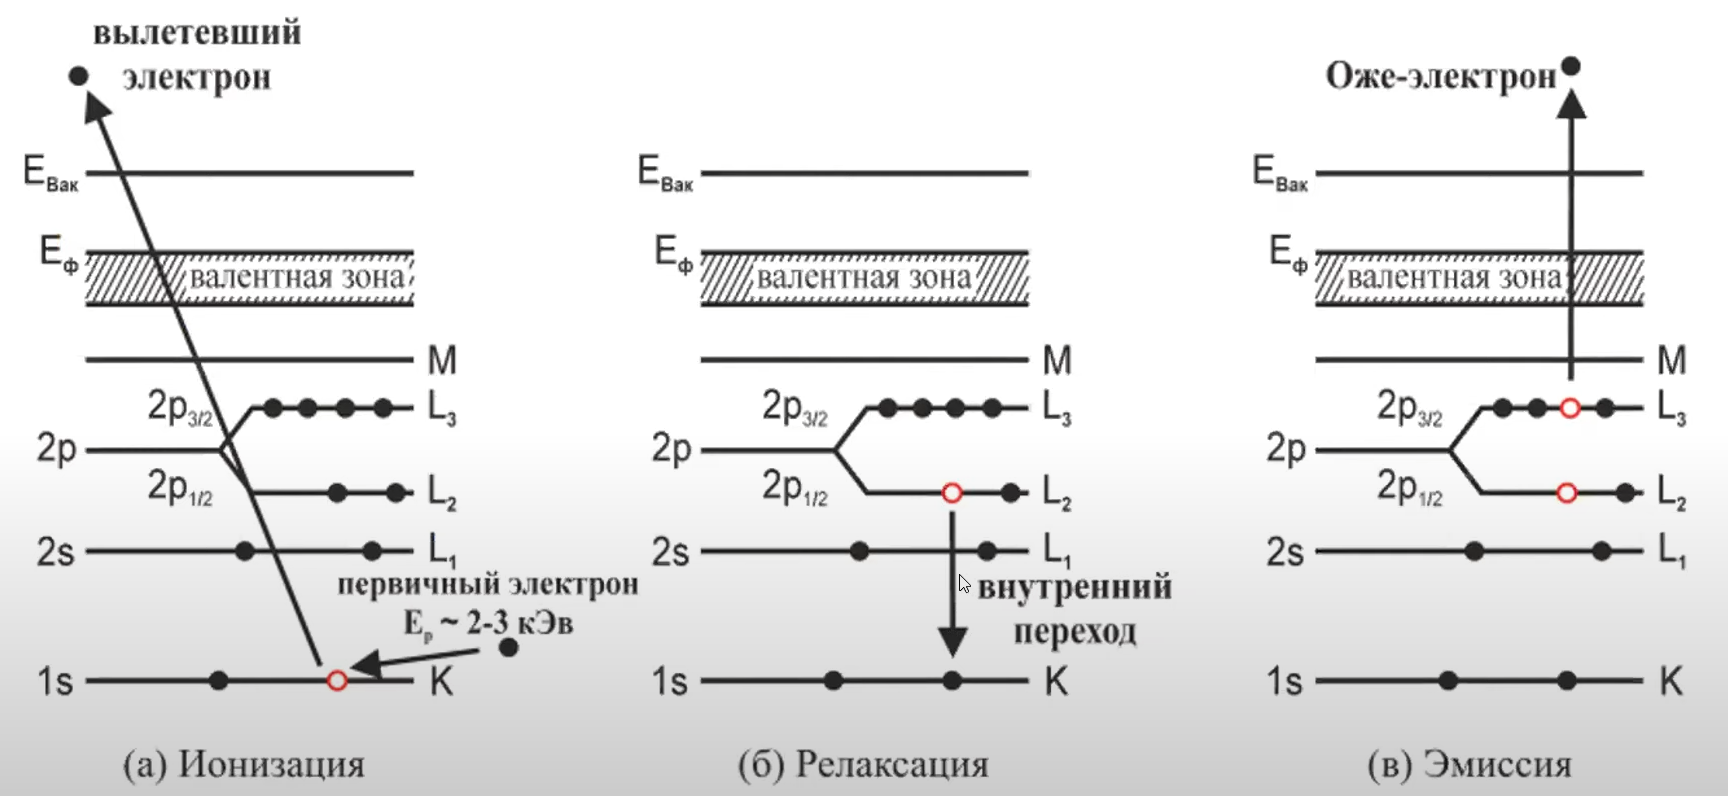
\includegraphics[width=0.7\linewidth]{1_diag}
		\caption{Схематическая иллюстрация оже-процесса из \cite{Auge_diag}.}
		\label{fig:1_diag}
	\end{figure}
	
	\subsection{Подготовка образца}
	
	Первоначально предлагалось закрепить образец на держателе с помощью танталовой нити с использованием контактной сварки, однако спустя несколько попыток было решено, что данный способ при отсутствии должной практики крайне сложен в практическом исполнении, принимая во внимание тот факт, что образец был цилиндрической формы. По этой причине было решено <<накрыть>> образец танталовой пластиной, предварительно просверлив в ней отверстие достаточного диаметра для получения Оже-спектра и сделав <<ножки>>, с помощью которых образец бы держался между пластинами.
	
	%\begin{figure}[H]
	%	\centering
	%	\includegraphics[width=0.7\linewidth]{1_fastening}
	%	\caption{Крепление образца с помощью танталовой пластины.}
	%	\label{fig:1_fastening}
	%\end{figure}
	
	\subsection{Анализ Оже-спектра}
	
	Изначально был получен Оже-спектр при бомбардировке образца электронами с энергией 3000~эВ с помощью установки, описанной в \cite{Auger_spectr}. С учетом возможности наличия т.н. пиков потерь, которые находятся в той же области, что и оже-пики, было решено проверить их присутствие с помощью увеличения энергии бомбардирующих электронов на 500~эВ. В таком случае Оже-пики, которые являются характеристикой вещества, должны были бы остаться на месте, а пики потерь --- сместиться. Из рисунка \ref{fig:1_Auge_double} видно, что смещения ни одного из пиков не наблюдается, что свидетельствует о том, что все пики являются оже-пиками.
	
	В силу совпадения оже-спектров анализ проводился только спектра 3000~эВ. Однако в более <<далекой>> по энергиям части спектра для того, чтобы лучше разрешить пики, оказался полезен и спектр 3500~эВ. Понятно, что в идеале хотелось бы иметь спектр 5000~эВ, пики с которого соответствовали бы, как и пики с 3000~эВ, каталожным, однако это оказалось невозможно по независящим от нас техническим причинам. Проанализированный спектр 3000~эВ представлен на рисунке \ref{fig:1_Auge_3000}.
	
	Как было сказано, спектр 3500~эВ оказался полезен в <<дальней>> части спектра: с его помощью был уточнен пик, предположительно, тулия. Кроме того, благодаря тому, что это сканирование мы запустили с меньшего нижнего порога по энергиям, из него также можно было вытащить один дополнительный пик в начале, который оказался натриевым. Эти два ненайденных с помощью спектра 3000~эВ пика указаны на спектре 3500~эВ на рисунке \ref{fig:1_Auge_3500}. 
	
	В качестве каталожных спектров были взяты спектры из \cite{Auger}.
	
	\section{Сканирующая туннельная микроскопия}
	
	\subsection{Принцип метода}
	
	Сканирование осуществляется с помощью специальной очень острой металлической иглы, в идеале на крайней точке которого сидит один единственный атом. Если достаточно близко приблизить образец к игле и подать напряжение, то потечет туннельный ток, направление которого может меняться (с образца на иглу, или наоборот) в зависимости от полярности напряжения. По зависимости величины тока от напряжения можно получить информацию о расстоянии между зондом и атомами поверхности образца. Вероятность туннельного эффекта зависит экспоненциально от расстояния, что и обеспечивает высокое разрешение данного метода.
	
	Более полное описание микроскопа GPI-300, на котором проводилось сканирование, представлено в \cite{Eltsov}. Для сканирования, как было сказано выше, был выбран графитовый образец.
	
	\subsection{Измерение высоты ступеньки и получение обзорного СТМ-кадра}
	
	С помощью последовательного сканирования различных областей, была найдена область с несколькими ступенями. Полученное изображение представлено на рисунке \ref{fig:2_step}. График перепада высот на исследованной ступеньке указан на рисунке \ref{fig:2_step_anal}. Из последнего видно, что высота ступени определяется как $3.5$~\AA, что в целом соответствует данным, представленным, например, в \cite{Article}.
	
	\subsection{Наблюдение атомной структуры}
	
	На рисунке \ref{fig:2_atomic} представлено полученное СТМ-изображение поверхности графита с атомной модуляцией. Мы видим четкую гексагональную структуру решетки, которая образуется двумя атомными слоями графита, смещенными друг относительно друга. Наблюдаемый нами гексагон --- точки с максимальной электронной плотностью, т.е. те места, где узлы двух слоев (фиолетового и желтого) совпадают (см. схему на рисунке \ref{fig:2_atomic}). Зная, что мы должны наблюдать правильный гексагон, мы можем по теореме косинусов определить реальное расстояние между атомами одного слоя, зная расстояние между соседними наблюдаемыми модуляциями. Межатомное расстояние, посчитанное таким образом, оказывается равным $1.4$~\AA. 
	
	
	
	\subsection{Зависимость СТМ-изображения атомной структуры от напряжения}
	
	На одном и том же участке было проведено несколько последовательных сканирований при различных напряжениях с целью найти зависимость профиля изображения от напряжения. Полученные кадры представлены на рисунке \ref{fig:2_different_volt}, а профили одного из рядов на них --- на рисунке \ref{fig:2_different_volt_profiles}. Из последнего видно, что с увеличением напряжения ''глубина'' профиля становится все меньше. Это наблюдение подтверждается в \cite{STM_Binnig}.
	
	\subsection{Наблюдение муара}
	
	Увиденный нами муар представлен на рисунке \ref{fig:2_muar}. Наблюдаются атомные модуляции, а также модуляция сверхструктуры. На Фурье-образе также видно две структуры: атомный гексагон и гексагон сверхструктуры. Было вычислено расстояние между соседними элементами сверхструктуры, которое оказалось равным $7.64\text{ нм}/2 = 3.82$~нм. Реально было измерено расстояние не между двумя соседними элементами, а между элементами, находящимися через один, чтобы накопить большую статистику.
	
	Было высказано предположение, что муар составлен двумя ''слоями'' графита (''слои'' здесь подразумевают не один атомный слой, а объединение двух, см. пункт про атомную структуру). С помощью моделирования было установлена, что ''слои'' должны быть развернуты друг относительно друга на 6.2$^\circ$. Смоделированный муар представлен на рисунке \ref{fig:2_muar_model}.
	
	\section{Сканирующая туннельная спектроскопия}
	
	\subsection{Принцип метода}
	
	Согласно \cite{Mironov} скажем, что выражения для туннельного тока может быть представлено в следующем виде:
	
	\begin{equation}
		dI = A \cdot D(E) \rho_P (E) f_P(E) \rho_S(E)(1 - f_S(E)) dE
	\end{equation}
	
	Здесь $A$ --- некоторая постоянная, $D(E)$ --- прозрачность барьера, $\rho_P(E), \rho_S(E)$ --- плотности состояний в материале зонда и исследуемого образца соответственно, $f(E)$ --- функция распределения Ферми.
	
	Предполагая, что плотность состояний вблизи уровня ферми в зонде практически постоянна, а также предполагая, что температуры низкие, мы можем записать:
	
	\begin{equation}
		I(V) \propto \int\limits_0^{eV} \rho_S(E)dE 
	\end{equation} 
	
	Тогда зависимость туннельного тока от напряжения определяется плотностью состояний в энергетическом спектре образца. Тогда для плотности состояний мы можем записать:
	
	\begin{equation}
		\rho_S(eV) \propto \frac{\partial I}{\partial V}
	\end{equation}
	
	То есть на деле, снимая ВАХ, а затем дифференцируя ее, мы можем судить о плотности состояний в исследуемом образце.
	
	\subsection{Снятие ВАХ}
	
	На уже использованном для СТМ графитовом образце было снято несколько ВАХ на одном и том же месте. После анализа результатов была выбрана наименее зашумленная серия, которая после этого была дополнительно отфильтрована. Полученная ВАХ (исходная и после фильтра) представлена на рисунке \ref{fig:3_STS}. Видно, что на ней все еще достаточно много шумов. Чтобы это улучшить, вероятно, стоит изначально подводить иглу ближе к образу (т.е. менять $U_{\text{base}}$), а также уменьшить шаг по напряжению.
	
	\section{Выводы}
	
	В результате проведения лабораторной работы:
	
	\begin{enumerate}
		\item Был расшифрован Оже-спектр неизвестного образца. Предположительно он состоит из натрия, фтора, тулия и иттрия. Принимается, что пики углерода и кислорода происходят из остатков газа в вакуумной камере.
		
		\item Была получен обзорный СТМ-кадр с моноатомной ступенькой. Была измерена ее высота, которая оказалась равной 3.5~\AA, что согласуется с указанным в \cite{Article}.
		
		\item Был получен СТМ-кадр атомной структуры, из которого после анализа было получено межатомное расстояние в решетке графита: 1.4~\AA.
		
		\item Был проведен эксперимент по поиску зависимости СТМ-изображения атомной структуры от напряжения, в ходе которого было установлено, что с ростом напряжения ''глубина'' кадра уменьшается, что подтверждается в \cite{STM_Binnig}.
		
		\item При сканировании был обнаружен муар, который, по всей видимости, вызывается поворотом двух (или более) ''слоев'' решетки относительно друг друга. В результате компьютерного моделирования этого предположения было установлено, что в таком случае слои должны быть повернуты друг относительно друга на $6.2^\circ$.
		
		\item Была получена ВАХ, которая отдаленно напоминает ВАХ, например, из \cite{Article}, однако она сильно зашумлена. В качестве вариантов решения проблемы в будущем были предложены более близкое подведение иглы к образцу и уменьшение шага по напряжению.
	\end{enumerate}
	
	\newpage
	
	\begin{thebibliography}{2}
		
		\bibitem{Auger} Handbook of Auger Electron Spectroscopy. /  Lawrence E. Davis, Noel C. MacDonald, Paul W. Palmberg, Greald E. Riach, Roland E. Wever --- Physical Electrinics Industries, Inc., February 1976.
		
		\bibitem{Auger_spectr} Описание работы оже-спектрометра. / ??
		
		\bibitem{STM} Общее описание СТМ GPI-300. / ??
		
		\bibitem{Article} Scanning tunneling microscopy and spectroscopy of the electronic local density of states of graphite surfaces near monoatomic step edges. / Y. Niimi, T. Matsui, H. Kambara, K. Tagami, M. Tsukada, and Hiroshi Fukuyama --- Tokyo, Japan : Department of Physics, University of Tokyo, February 24, 2006.
		
		\bibitem{Auge_diag} Анализ поверхности методами Оже- и рентгеновской фотоэлектронной спектроскопии. / Бриггса Д., Сиха М.М.
		
		\bibitem{Eltsov} Сверхвысоковакуумный сканирующий туннельный микроскоп GPI-300. / Ельцов К.Н. , А.Н. Климов, А.Н. Косяков, О.В. Объедков, В.Ю. Юров, В.М. Шевлюга --- Москва : Труды института общей физики им. А.М. Прохорова, 2003.
		
		\bibitem{Mironov} Основы сканирующей зондовой микроскопии. / В.Л. Миронов --- Нижний Новгород : Институт физики микроструктур, 2004
		
		\bibitem{STM_Binnig} Binnig, Gerd, and Heinrich Rohrer. ''Scanning tunneling microscopy.'' IBM Journal of research and development 44.1/2 (2000): 279.
		
	\end{thebibliography}
	
	
	\newpage
	
	% Оже-спектры выношу отдельно, по одному на страницу, чтобы не сидеть "а че там написано"
	
	\begin{figure}[H]
		\centering
		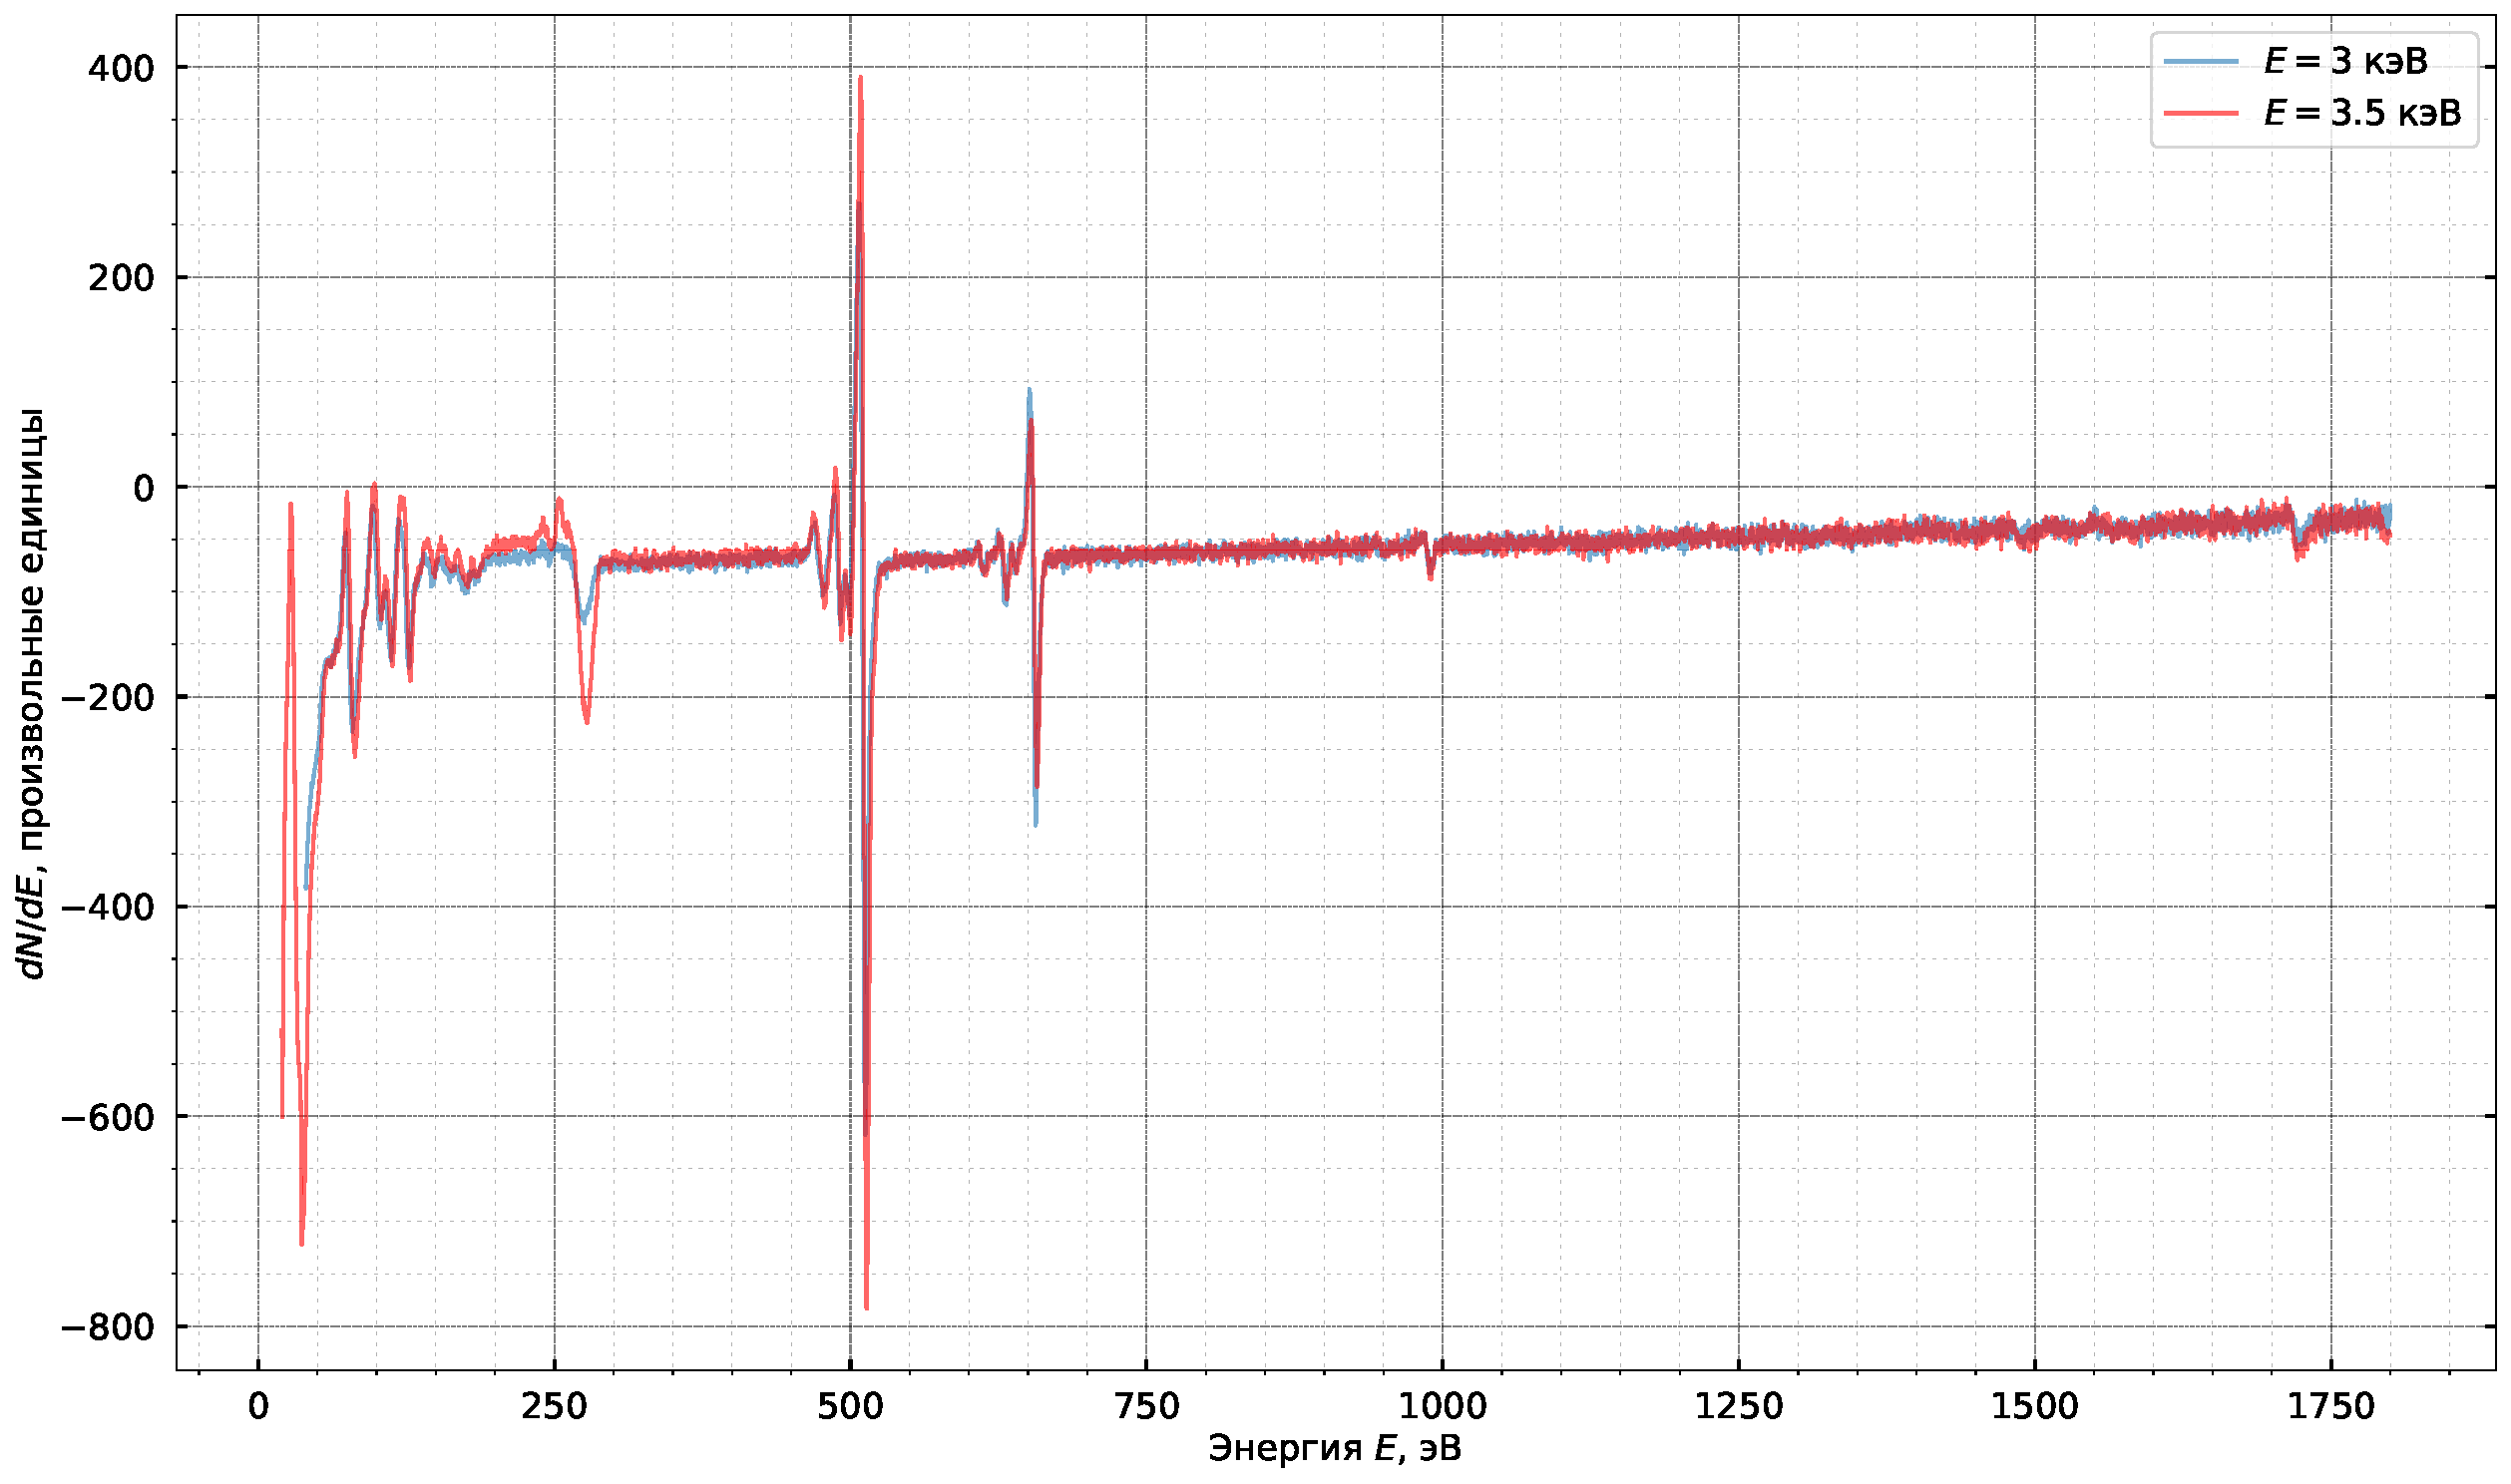
\includegraphics[width=1.3\linewidth, angle=-90]{1_Auge_double}
		\caption{Сравнение Оже-спектров, полученных при 3000~эВ и 3500~эВ.}
		\label{fig:1_Auge_double}
	\end{figure}
	
	\newpage
	
	\begin{figure}[H]
		\centering
		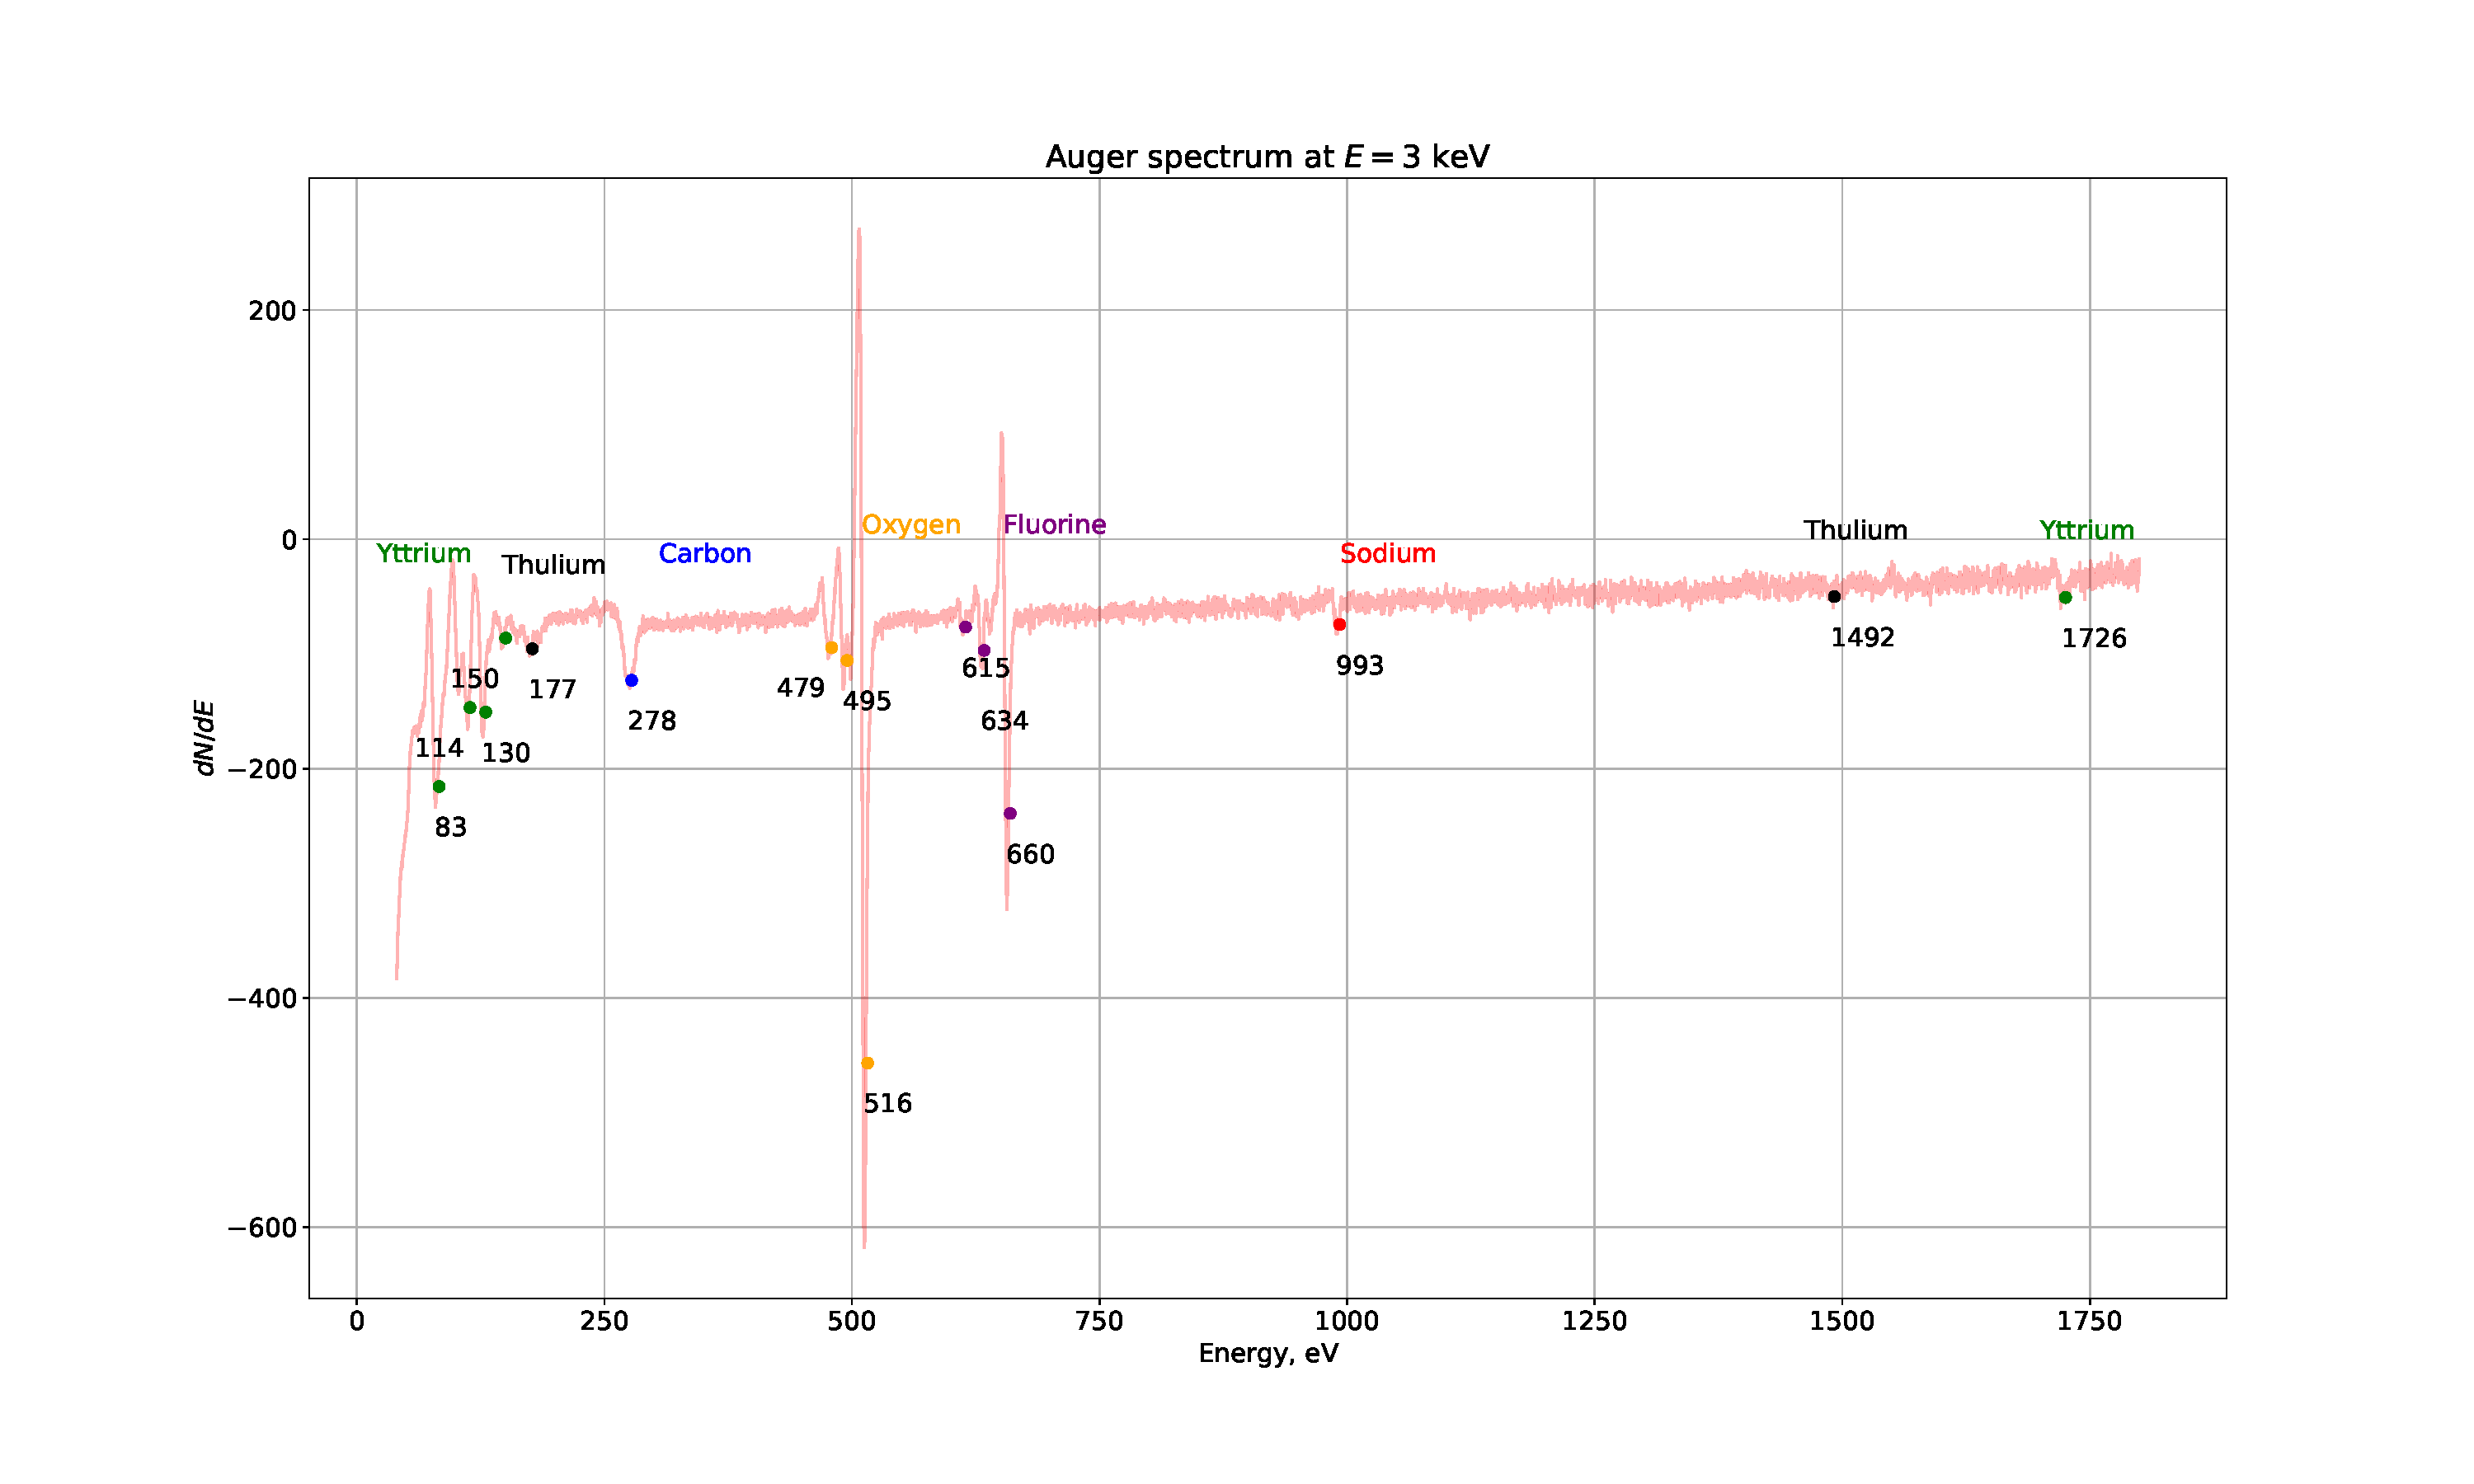
\includegraphics[width=1.3\linewidth, angle=-90]{1_Auge_3000}11
		\caption{Полученный Оже-спектр 3000~эВ с нанесенными названиями элементов, дающих пики.}
		\label{fig:1_Auge_3000}
	\end{figure}
	
	\newpage
	
	\begin{figure}[H]
		\centering
		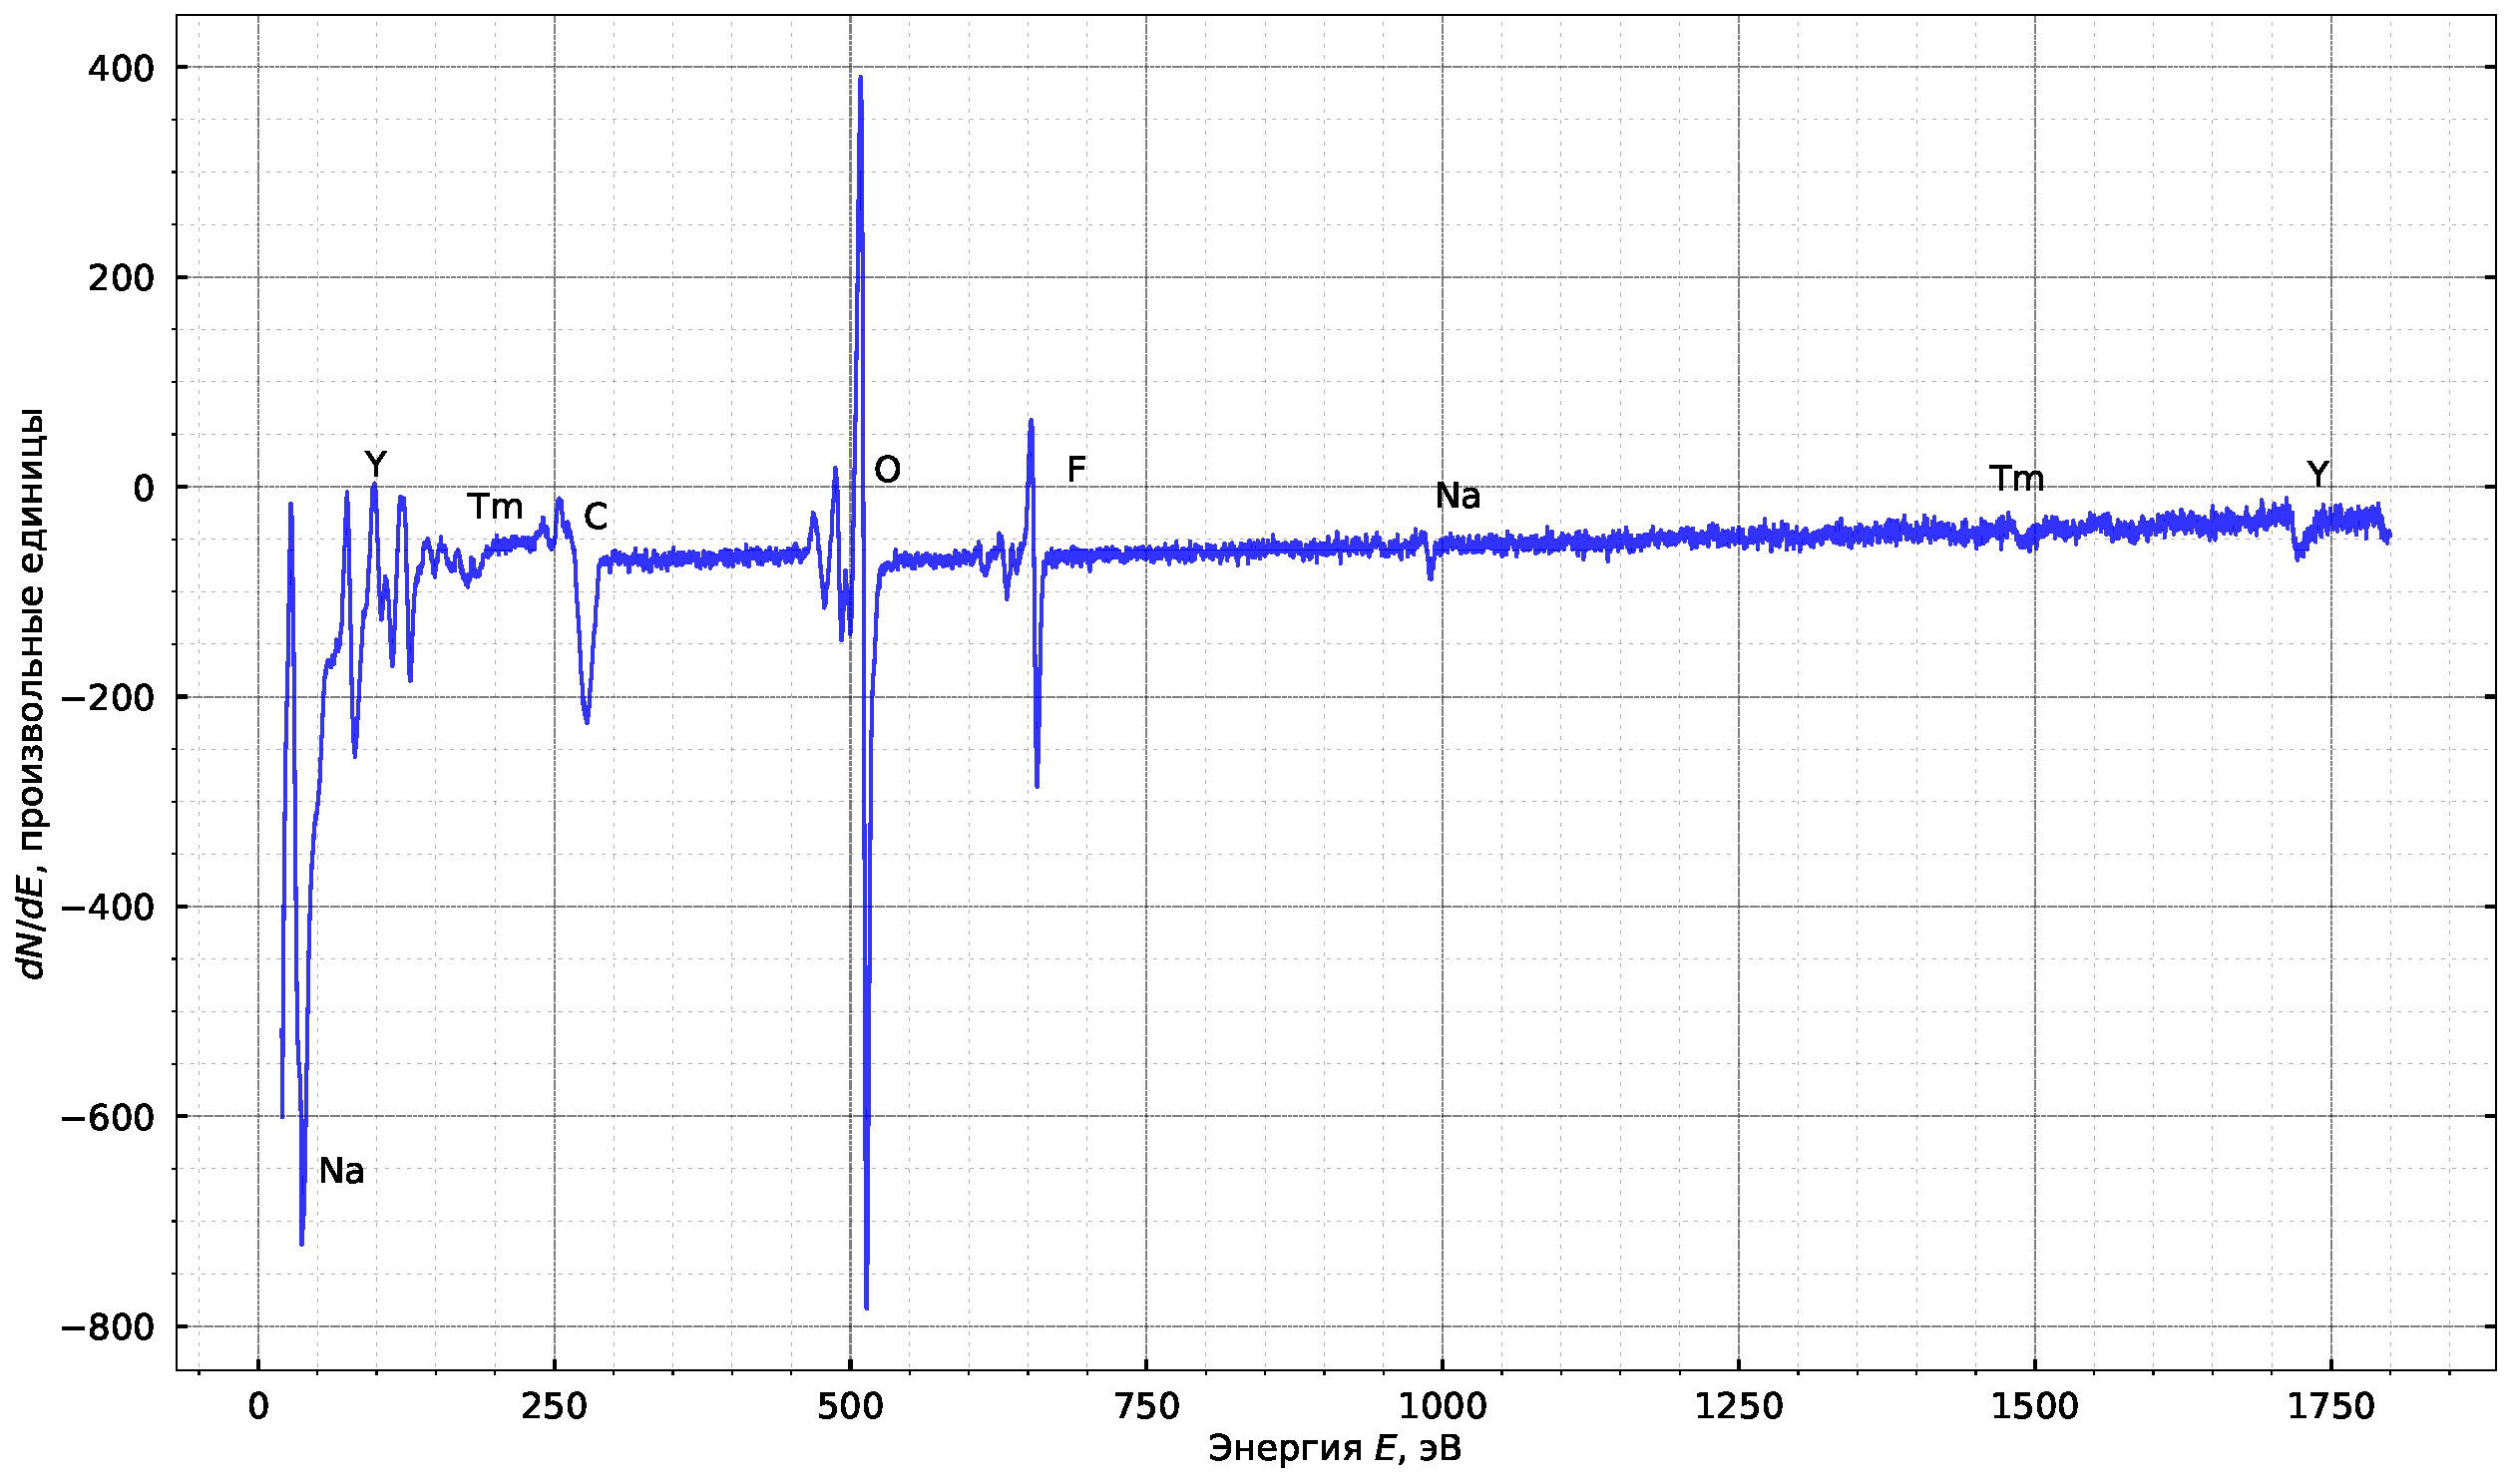
\includegraphics[width=1.3\linewidth, angle=-90]{1_Auge_3500}
		\caption{Полученный Оже-спектр 3000~эВ с нанесенными названиями элементов, дающих не найденные на 3000~эВ пики.}
		\label{fig:1_Auge_3500}
	\end{figure}
	
	\newpage
	
	\begin{figure}[H]
		\centering
		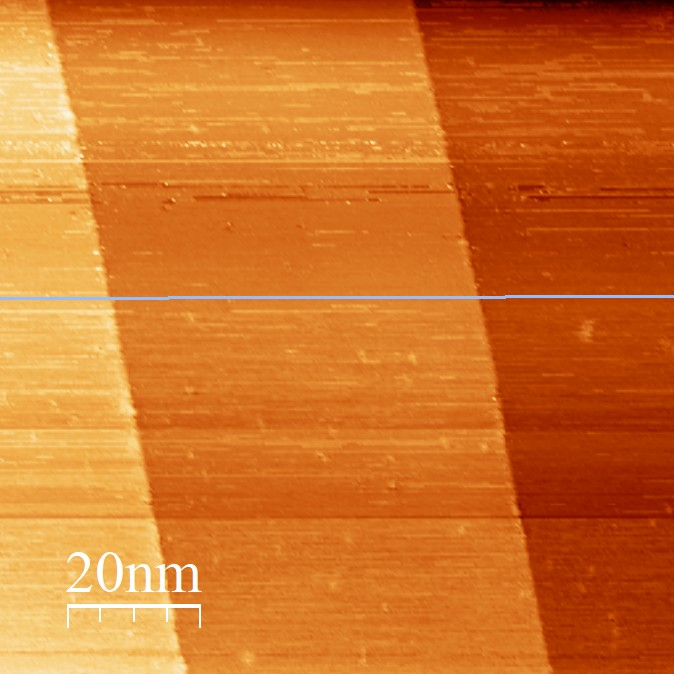
\includegraphics[width=0.58\linewidth]{../STM_data/Step/Step_final}
		\caption{Обзорный СТМ-кадр поверхности графита. Размер кадра $100\times100$~нм, ток 0.5~нА, напряжение 375~мВ.}
		\label{fig:2_step}
	\end{figure}
	
	\begin{figure}[H]
		\centering
		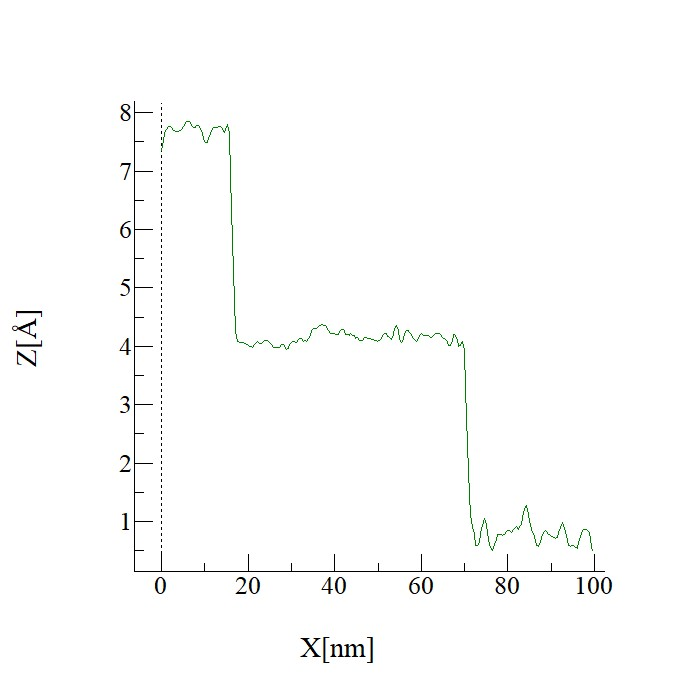
\includegraphics[width=0.6\linewidth]{../STM_data/Step/Step_final_Graph_enh.jpg}
		\caption{Профиль ступеньки графита, из которого видна высота ступеньки --- $3.5$~\AA.}
		\label{fig:2_step_anal}
	\end{figure}

	\begin{figure}[H]
		\centering
		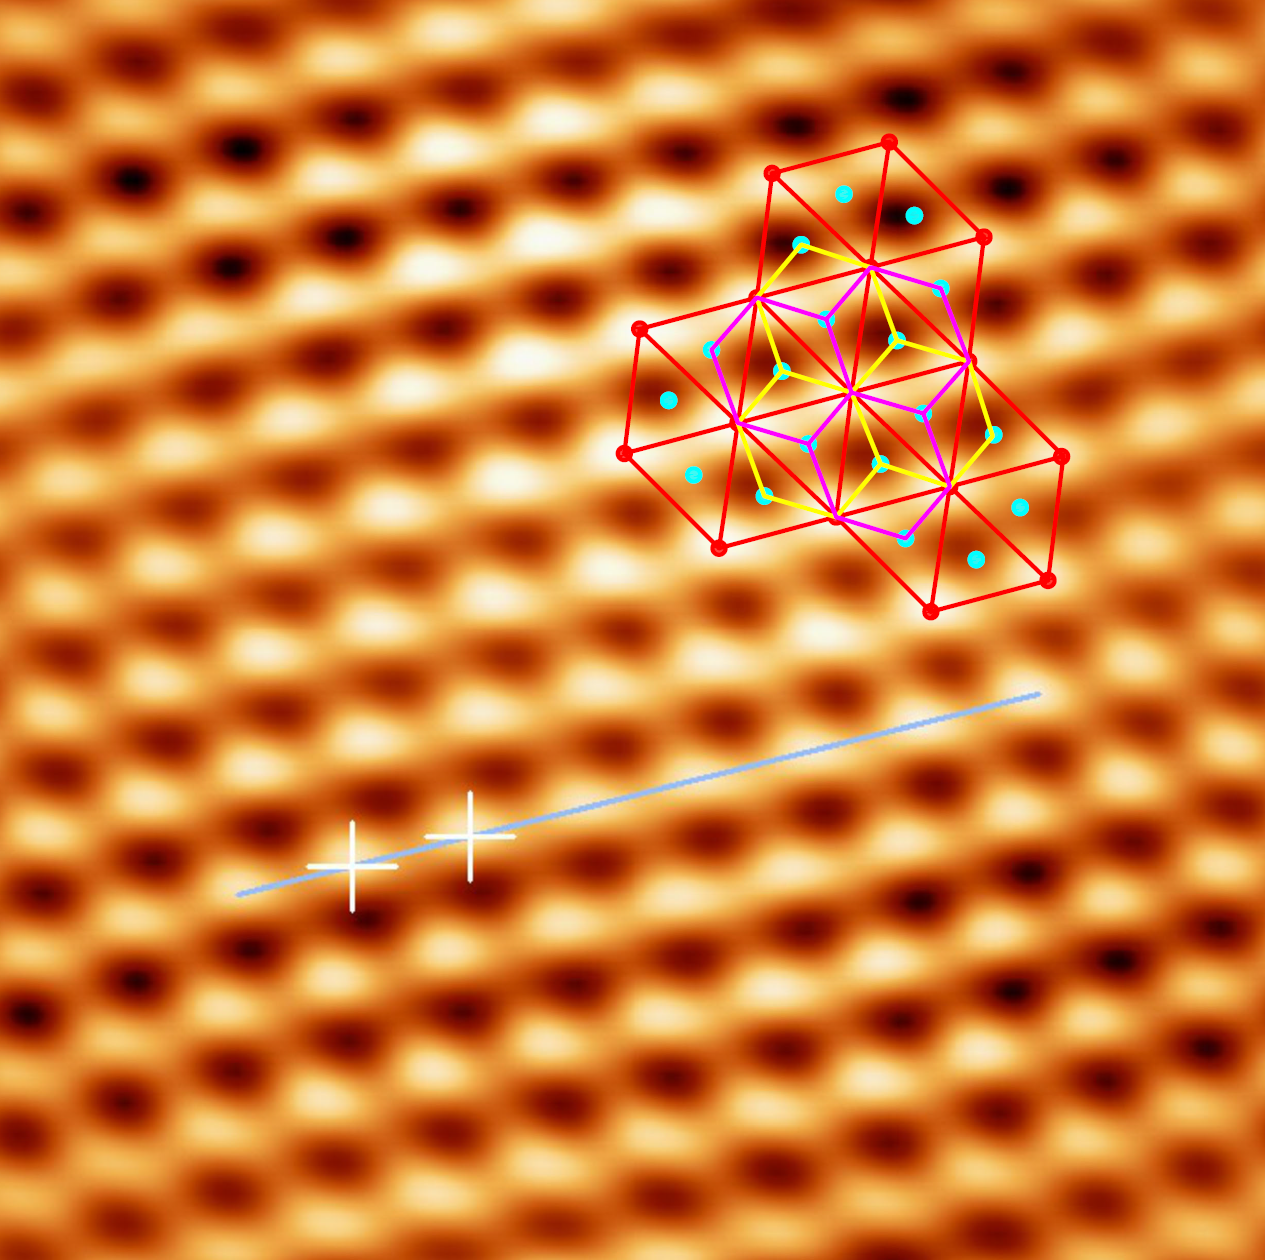
\includegraphics[width=0.6\linewidth]{../STM_data/Crystal_cell_structure/Crystal_structure_with_net}
		\caption{Атомная структура поверхности графита, размер кадра $2.6\times2.6$~нм, ток $0.4$~нА, напряжение 25.6~мВ, расстояние между двумя модуляциями 2.33~\AA. На кадр нанесены две решетки слоев графита, сдвинутых друг относительно друга, перекрытие которых дает наблюдаемую атомную модуляцию.}
		\label{fig:2_atomic}
	\end{figure}

	\begin{figure}[H]
		\centering
		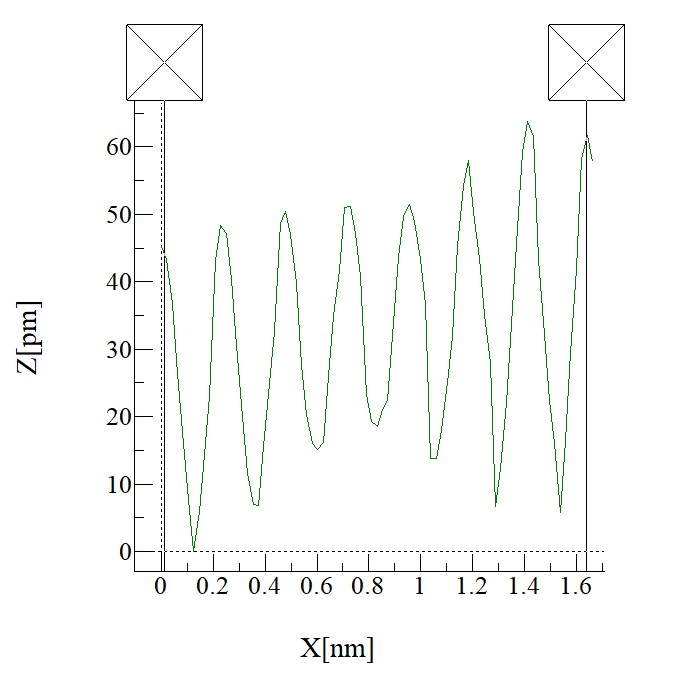
\includegraphics[width=0.5\linewidth]{../STM_data/Crystal_cell_structure/Crystal_structure_g}
		\caption{Профиль изображения \ref{fig:2_atomic}, из которого получается расстояние между модуляциями 2.33~\AA. Измерено расстояние между несколькими модуляциями для накопления большей статистики.}
		\label{fig:2_atomic_g}
	\end{figure}
	
	\begin{figure}[H]
		\centering
		\subfigure[]{
			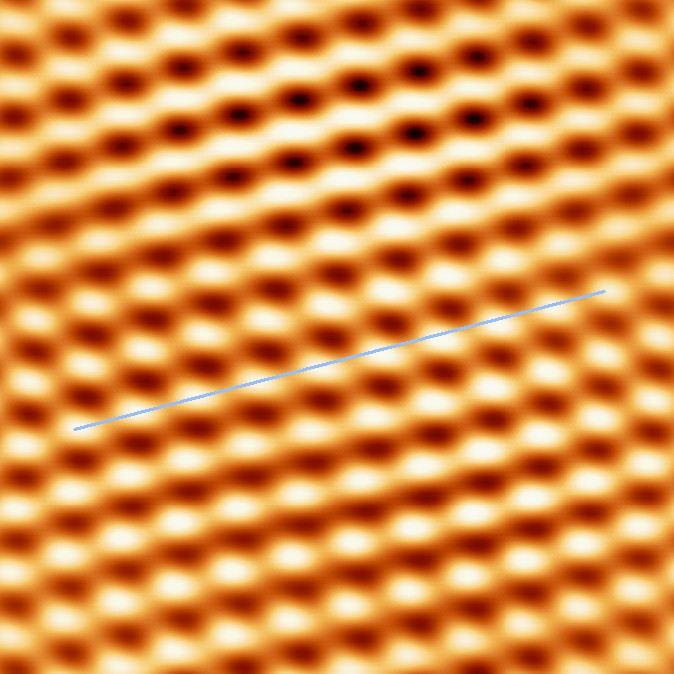
\includegraphics[width=0.36\linewidth]{../STM_data/STM_Profiles_new/Pictures/25_6_1}
		}	
		\subfigure[]{
			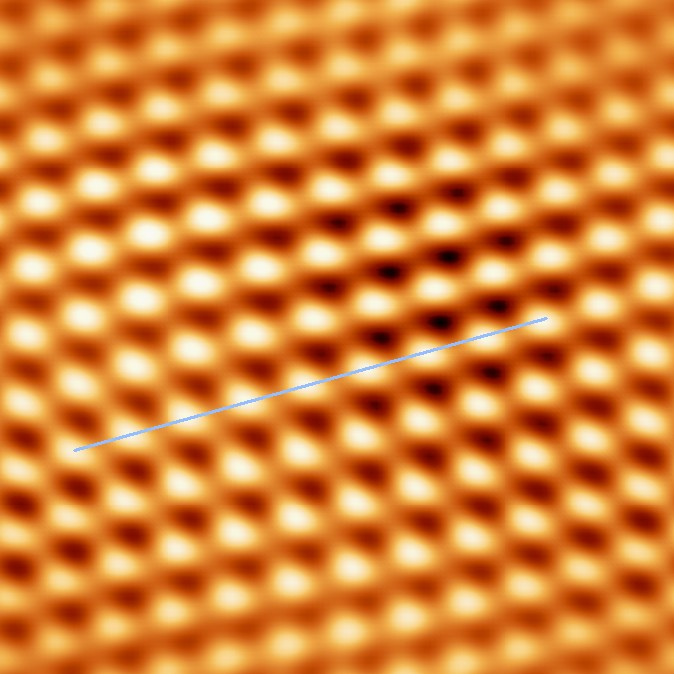
\includegraphics[width=0.36 \linewidth]{../STM_data/STM_Profiles_new/Pictures/64_4_1}
		}
		\subfigure[]{
			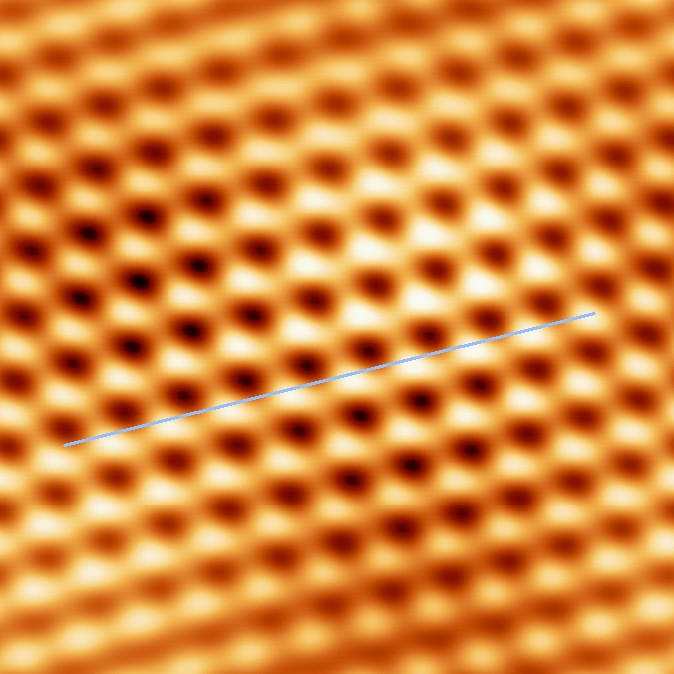
\includegraphics[width=0.36\linewidth]{../STM_data/STM_Profiles_new/Pictures/93_3_1}
		}	
		\subfigure[]{
			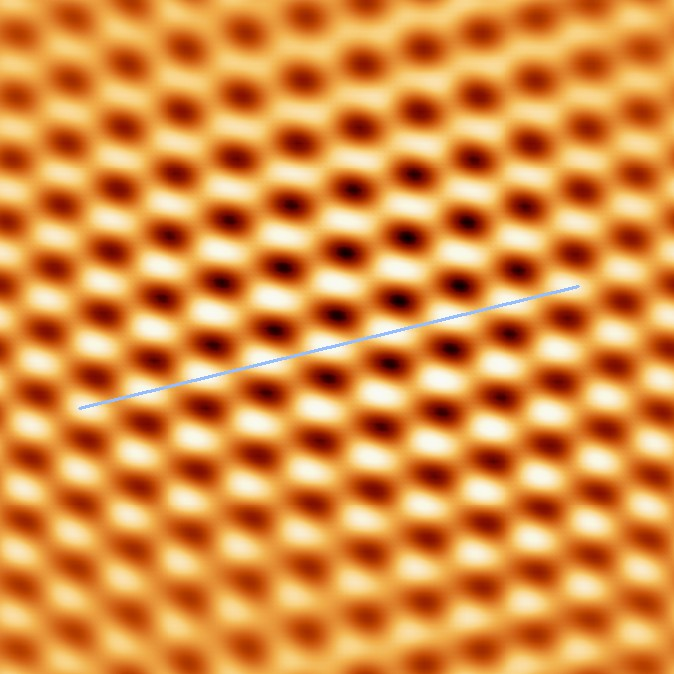
\includegraphics[width=0.36 \linewidth]{../STM_data/STM_Profiles_new/Pictures/150_1_1}
		}
		\subfigure[]{
			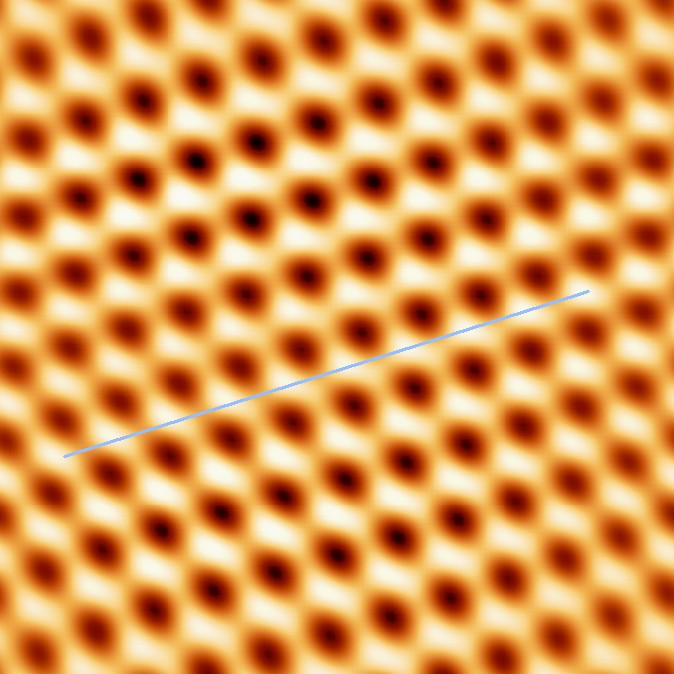
\includegraphics[width=0.36 \linewidth]{../STM_data/STM_Profiles_new/Pictures/200_1}
		}
		
		\caption{СТМ-изображение атомной структуры при различных напряжениях. Слева направо и сверху вниз при напряжении, соответственно: 25.6~мВ, 64.4~мВ, 93.3~мВ, 150.1~мВ, 200~мВ. Размеры всех изображений составляют $2.6\times2.6$~нм, ток --- 0.4~нА.}
		\label{fig:2_different_volt}
	\end{figure}

	\begin{figure}[H]
		\centering
		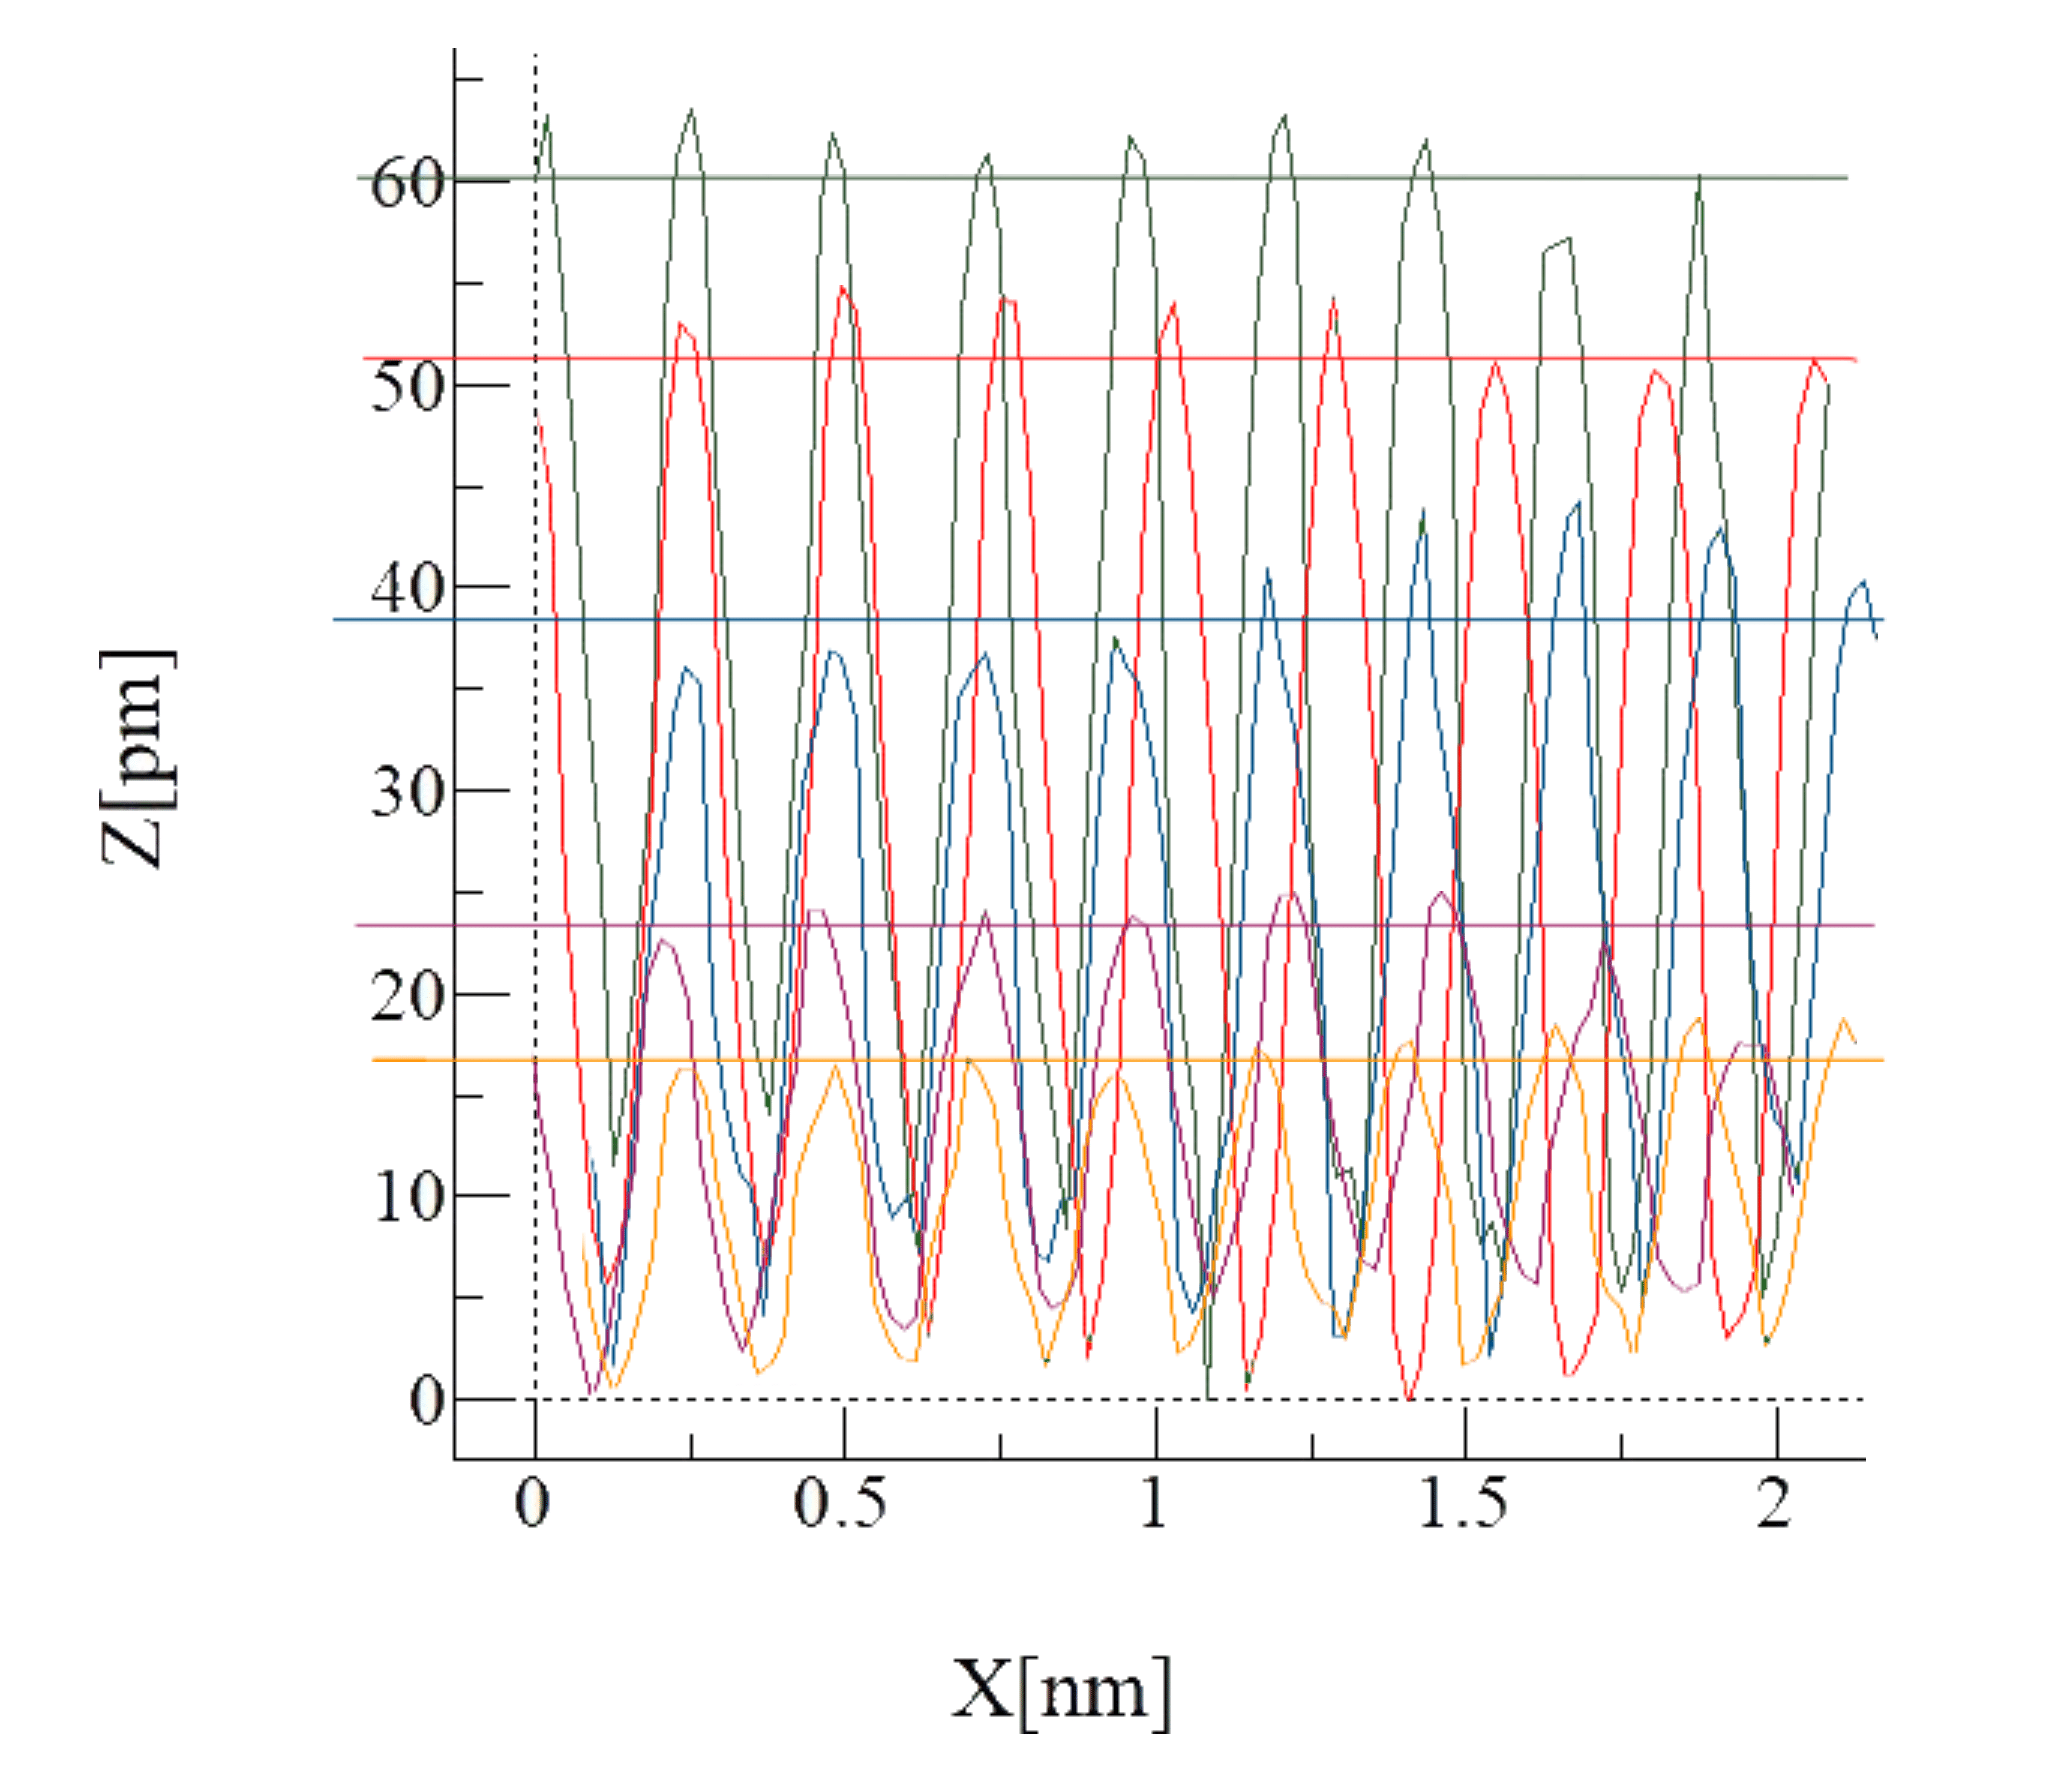
\includegraphics[width=0.9\linewidth]{../STM_data/STM_Profiles_new/Graphs/All_graphs}
		\caption{Профили атомного изображения при одинаковых токах (0.4~нА), но при различных напряжениях: зеленый --- 25.6~мВ, красный --- 64.4~мВ, синий --- 93.3~мВ, фиолетовый --- 150.1~мВ, оранжевый --- 200~мВ.}
		\label{fig:2_different_volt_profiles}
	\end{figure}
	
	\begin{figure}[H]
		\centering
		\subfigure[]{
			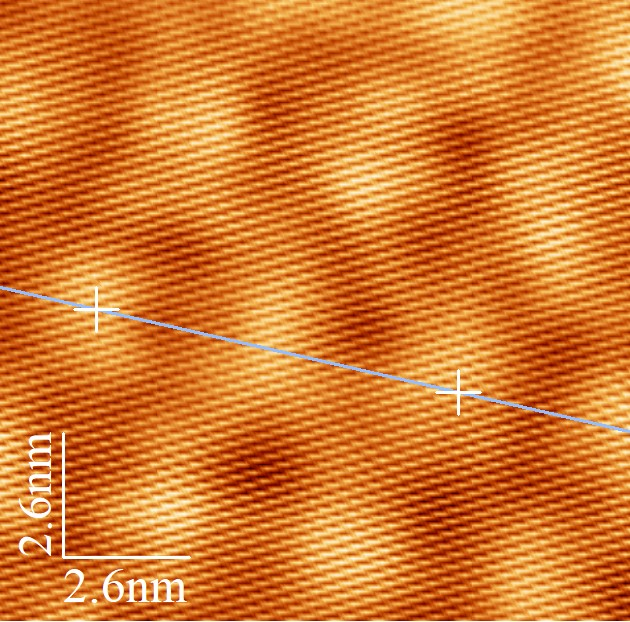
\includegraphics[width=0.45\linewidth]{../STM_data/Muar/Muar_final}
		}
		\subfigure[]{
			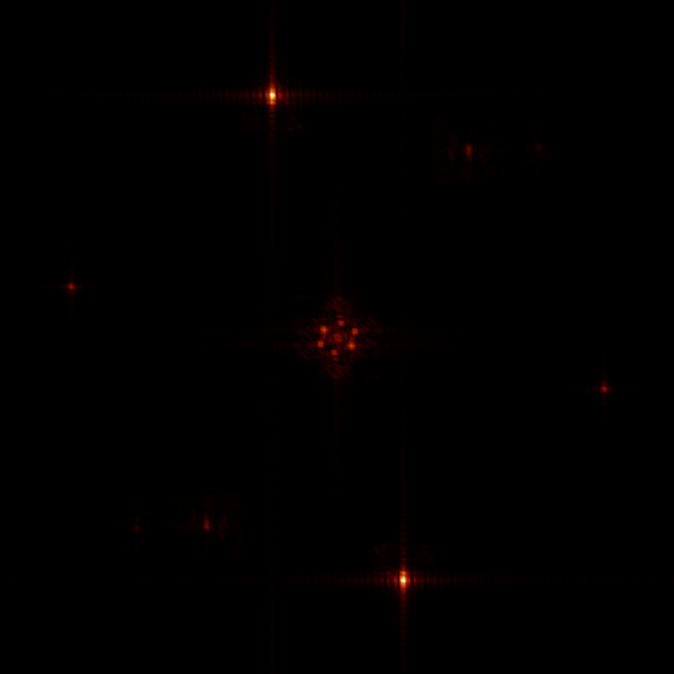
\includegraphics[width=0.45\linewidth]{../STM_data/Muar/Muar_final_f}
		}
		\subfigure[]{
			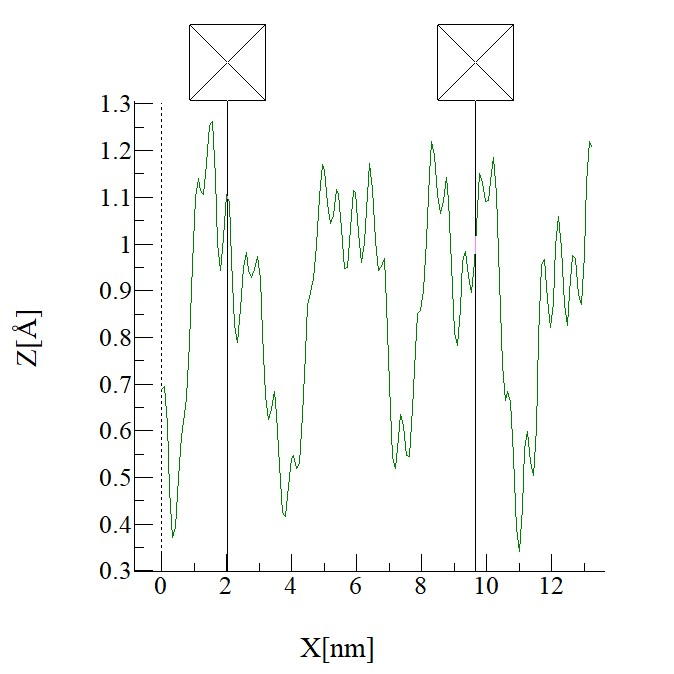
\includegraphics[width=0.6\linewidth]{../STM_data/Muar/Muar_final_g}
		}
		\caption{СТМ-кадр графита с наблюдающимся муаром, размер изображения $13\times13$~нм, ток 0.3~нА, напряжение 297~мВ (a), его Фурье-образ (b), профиль для определения расстояния между элементами сверхструктуры, оказавшегося равным 3.82~нм (c).}
		\label{fig:2_muar}
	\end{figure}

	\begin{figure}[H]
		\centering
		
\includegraphics[width=0.9\linewidth]{../STM_data/Muar/Muar_model}
		\caption{Компьютерное моделирование сверхструктуры.}
		\label{fig:2_muar_model}
	\end{figure}
	
	\begin{figure}[H]
		\centering
		\subfigure[]{
			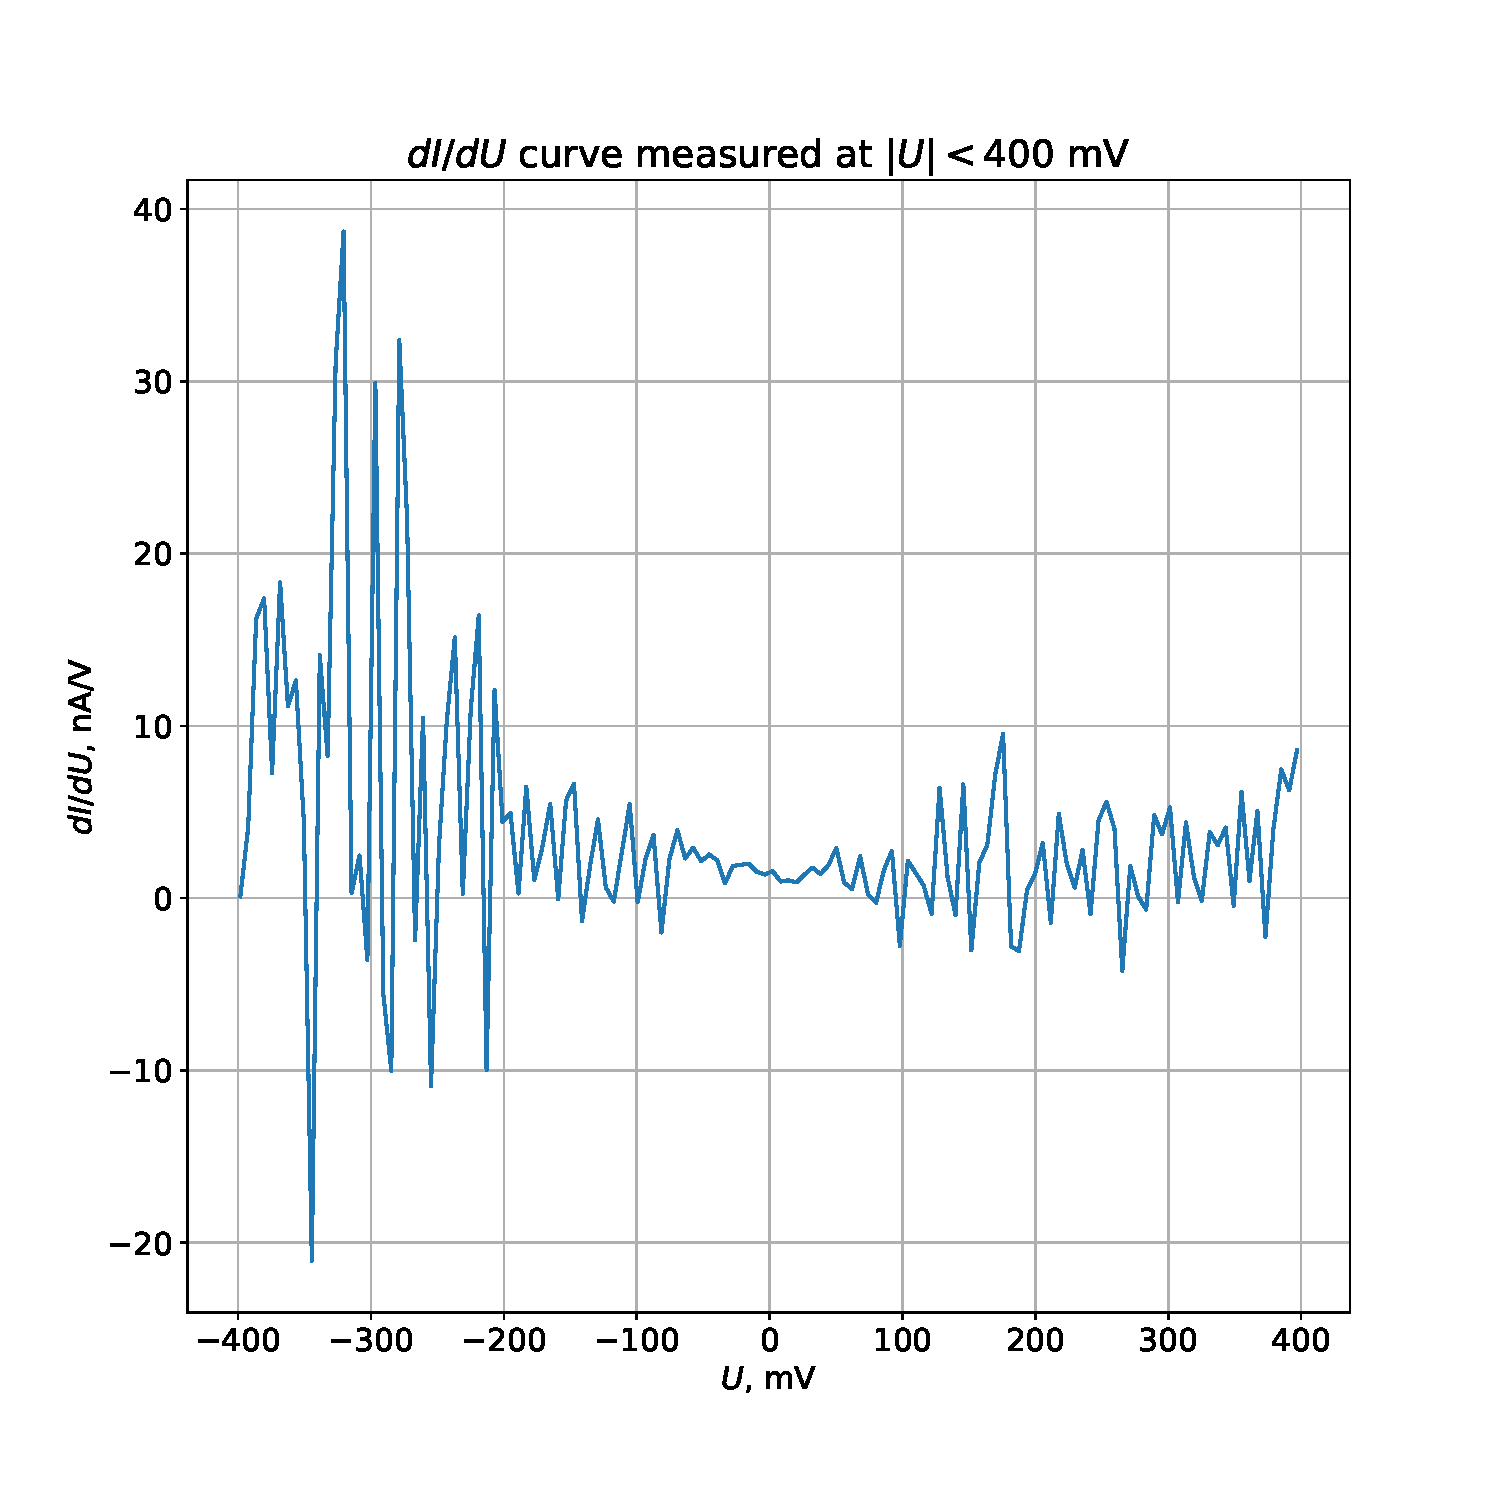
\includegraphics[width=0.6\linewidth]{3_curve}
		}
		\subfigure[]{
			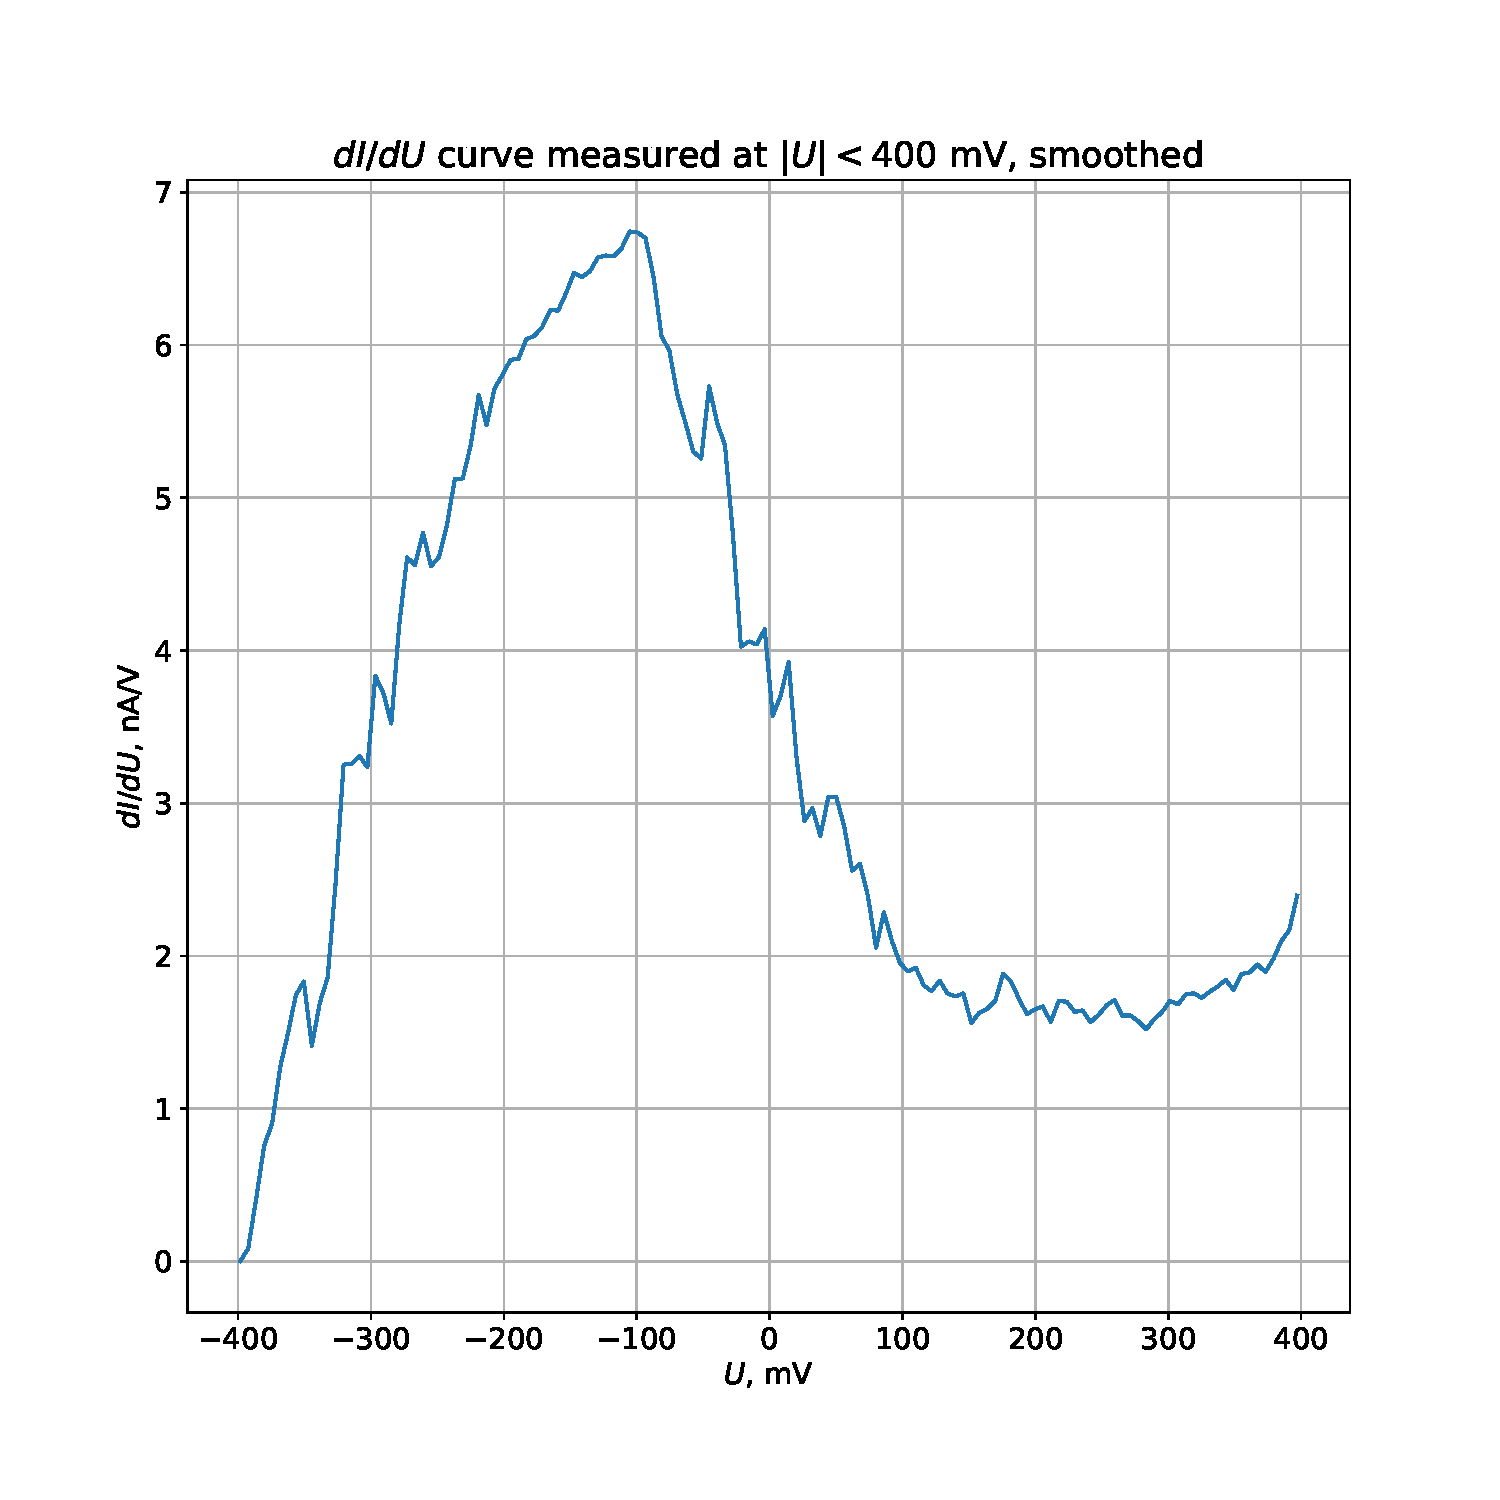
\includegraphics[width=0.6\linewidth]{3_curve_smooth}
		}
		\caption{Кривая $dI/dU$, измеренная при $|U| < 400$~mV (сверху) и она же, пропущенная через фильтр (снизу).}
		\label{fig:3_STS}
	\end{figure}
	
	
	
	
	
	
	
	
	
	
	
	
	
	
	
	
	
	
	
	
	
	
	
	
	
	
	
	
	
	
	
	
	
	
\end{document}